\documentclass[12pt,a4paper]{article}

% ============================================================
% PACKAGES
% ============================================================
\usepackage[utf8]{inputenc}
\usepackage[T1]{fontenc}
\usepackage[french]{babel}
\usepackage{geometry}
\geometry{top=2.5cm, bottom=2.5cm, left=2.5cm, right=2.5cm}
\usepackage{graphicx}
\usepackage{float}
\usepackage{booktabs}
\usepackage{array}
\usepackage{xcolor}
\usepackage{colortbl}
\usepackage{hyperref}
\usepackage{fancyhdr}
\usepackage{titlesec}
\usepackage{enumitem}
\usepackage{tcolorbox}
\usepackage{caption}
\usepackage{tabularx}
\usepackage{lastpage}
\usepackage{pdflscape}

% ============================================================
% COULEURS
% ============================================================
\definecolor{bleuTBM}{RGB}{41,128,185}
\definecolor{grisFonce}{RGB}{44,62,80}
\definecolor{grisClair}{RGB}{236,240,241}
\definecolor{bleuClair}{RGB}{235,245,251}

% ============================================================
% CONFIGURATION
% ============================================================
\hypersetup{
    colorlinks=true,
    linkcolor=bleuTBM,
    urlcolor=bleuTBM,
    pdftitle={Analyse des dynamiques de mobilité urbaine à Bordeaux},
    pdfauthor={Projet Data Visualisation \#2}
}

% En-tête et pied de page
\pagestyle{fancy}
\fancyhf{}
\fancyhead[L]{\small\textit{Rapport -- Analyse de Mobilité Urbaine à Bordeaux}}
\fancyhead[R]{\small\textit{Page \thepage\ / \pageref{LastPage}}}
\fancyfoot[C]{\small\textit{Projet Data Visualisation \#2 -- TBM Bordeaux -- Mars 2026}}
\renewcommand{\headrulewidth}{0.5pt}
\renewcommand{\footrulewidth}{0.3pt}

% Style des sections
\titleformat{\section}{\Large\bfseries\color{bleuTBM}}{}{0em}{}[\titlerule]
\titleformat{\subsection}{\large\bfseries\color{grisFonce}}{}{0em}{}

% Chemin des images
\graphicspath{{../visualisations/}}

% Encadré info
\newtcolorbox{infobox}[1][]{
    colback=bleuClair,
    colframe=bleuTBM,
    fonttitle=\bfseries\color{bleuTBM},
    title=#1,
    boxrule=0.5pt,
    arc=2pt,
    left=8pt, right=8pt, top=5pt, bottom=5pt
}

% ============================================================
% DOCUMENT
% ============================================================
\begin{document}

% ============================================================
% PAGE DE GARDE
% ============================================================
\begin{titlepage}

% Logo EPSI en haut à droite
\begin{flushright}
\includegraphics[width=4cm]{epsi (1).png}
\end{flushright}

\vspace{-1cm}

\begin{center}

\vspace*{1cm}

\colorbox{bleuTBM}{%
\parbox{0.9\textwidth}{%
\centering\vspace{1cm}
{\Huge\bfseries\color{white} ANALYSE DES DYNAMIQUES\\[0.3cm] DE MOBILITÉ URBAINE}\\[0.8cm]
{\Large\color{white} à partir des données de transport public}\\[0.5cm]
\rule{0.4\textwidth}{1pt}\\[0.5cm]
{\LARGE\bfseries\color{white} BORDEAUX MÉTROPOLE (TBM)}
\vspace{1cm}
}}

\vspace{2cm}

{\Large\bfseries Projet Data Visualisation \#2}

\vspace{1cm}

{\large\bfseries Réalisé par :}\\[0.3cm]
{\large Yassine ZOUITNI}\\[0.2cm]
{\large Samuel RESSIOT}

\vspace{1.5cm}

{\large Date : 16 mars 2026}\\[0.3cm]
{\large Source : Transports Bordeaux Métropole (TBM)}\\[0.3cm]
{\large Format : GTFS (General Transit Feed Specification)}

\vspace{2cm}

\fcolorbox{bleuTBM}{grisClair}{%
\parbox{0.8\textwidth}{%
\centering\vspace{0.5cm}
{\large\bfseries\color{bleuTBM} CHIFFRES CLÉS}\\[0.4cm]
{\normalsize 2\,195\,275 passages analysés ~|~ 3\,957 arrêts ~|~ 133 lignes ~|~ 57\,084 trajets}\\[0.2cm]
{\normalsize 17 visualisations générées (12 PNG + 5 HTML interactifs)}\\[0.2cm]
{\normalsize 3 modèles prédictifs (Régression Linéaire, Random Forest, Gradient Boosting)}
\vspace{0.5cm}
}}

\end{center}
\end{titlepage}

% ============================================================
% TABLE DES MATIÈRES
% ============================================================
\tableofcontents
\newpage

% ============================================================
% 1. INTRODUCTION ET PROBLÉMATIQUE
% ============================================================
\section{Introduction et Problématique}

Ce projet s'inscrit dans le cadre du Projet Data Visualisation \#2, dont l'objectif est d'analyser les dynamiques de mobilité urbaine à partir des données de transport public. L'analyse porte sur la ville de Bordeaux, en utilisant les données GTFS (General Transit Feed Specification) fournies par TBM (Transports Bordeaux Métropole).

\subsection{Problématique}

La problématique centrale de ce projet est la suivante :

\begin{infobox}[Problématique]
Quels sont les schémas temporels et géographiques de la fréquentation des transports publics ? Quelles zones et lignes connaissent des surcharges ou des creux ? Quels scénarios d'optimisation des lignes ou des horaires peuvent être proposés ?
\end{infobox}

\subsection{Questions Spécifiques}

\begin{itemize}[leftmargin=2cm]
    \item Quels sont les horaires de pointe les plus critiques ?
    \item Quelles stations ou lignes nécessitent une extension ou une optimisation ?
    \item Comment la fréquentation varie-t-elle géographiquement ?
    \item Quels types de transport sont les plus utilisés ?
    \item Peut-on prédire l'affluence future à partir des tendances observées ?
\end{itemize}

\subsection{Objectifs du Projet}

\begin{itemize}[leftmargin=2cm]
    \item Collecter et nettoyer les données GTFS de Bordeaux Métropole
    \item Identifier les patterns temporels de fréquentation (heures de pointe, creux)
    \item Analyser la répartition géographique des arrêts et leur utilisation
    \item Créer des visualisations avancées (heatmaps, cartes, dashboards)
    \item Développer des modèles prédictifs d'affluence
    \item Formuler des recommandations d'optimisation du réseau
\end{itemize}

% ============================================================
% 2. DONNÉES UTILISÉES
% ============================================================
\newpage
\section{Données Utilisées}

\subsection{Source des Données}

Les données proviennent de TBM (Transports Bordeaux Métropole) et sont au format GTFS (General Transit Feed Specification). Ce format standardisé décrit les horaires et les itinéraires des transports en commun. Les données ont été téléchargées depuis la plateforme Mobility Database (\url{https://mobilitydatabase.org}).

\subsection{Fichiers GTFS chargés}

\begin{table}[H]
\centering
\begin{tabular}{|l|l|l|}
\hline
\rowcolor{bleuTBM} \textcolor{white}{\textbf{Fichier}} & \textcolor{white}{\textbf{Description}} & \textcolor{white}{\textbf{Contenu}} \\
\hline
agency.txt & Information sur l'opérateur & TBM Bordeaux \\
\hline
\rowcolor{grisClair} stops.txt & Liste de tous les arrêts & 3\,957 arrêts \\
\hline
routes.txt & Lignes de transport & 133 lignes \\
\hline
\rowcolor{grisClair} trips.txt & Trajets planifiés & 57\,084 trajets \\
\hline
stop\_times.txt & Horaires à chaque arrêt & 2\,195\,275 passages \\
\hline
\rowcolor{grisClair} calendar.txt & Calendrier des services & Jours de service \\
\hline
calendar\_dates.txt & Exceptions calendrier & Jours spéciaux \\
\hline
\rowcolor{grisClair} shapes.txt & Tracés des lignes & Géométrie des parcours \\
\hline
\end{tabular}
\caption{Fichiers GTFS utilisés dans l'analyse}
\end{table}

\subsection{Statistiques Globales des Données}

\begin{infobox}[Résumé des données analysées]
\begin{itemize}[leftmargin=0.5cm]
    \item Total de passages analysés : \textbf{2\,195\,275}
    \item Nombre d'arrêts uniques : \textbf{3\,957}
    \item Nombre de lignes de transport : \textbf{133}
    \item Nombre de trajets planifiés : \textbf{57\,084}
    \item Couverture horaire : 0h -- 23h (24 heures)
\end{itemize}
\end{infobox}

% ============================================================
% 3. MÉTHODOLOGIE
% ============================================================
\newpage
\section{Méthodologie}

\subsection{Architecture du Projet}

Le projet est structuré de manière modulaire, avec une séparation claire des responsabilités entre les différents composants. Chaque module a un rôle spécifique dans le pipeline d'analyse :

\begin{table}[H]
\centering
\begin{tabular}{|l|l|l|}
\hline
\rowcolor{bleuTBM} \textcolor{white}{\textbf{Module}} & \textcolor{white}{\textbf{Rôle}} & \textcolor{white}{\textbf{Technologies}} \\
\hline
data\_loader.py & Chargement des fichiers GTFS & Pandas \\
\hline
\rowcolor{grisClair} preprocessor.py & Nettoyage et enrichissement & Pandas, NumPy \\
\hline
analyzer.py & Analyse exploratoire & Pandas, NumPy \\
\hline
\rowcolor{grisClair} visualizer.py & Création des graphiques & Matplotlib, Seaborn, Plotly, Folium \\
\hline
predictor.py & Modélisation prédictive & Scikit-learn \\
\hline
\rowcolor{grisClair} main.py & Orchestration du pipeline & Python \\
\hline
\end{tabular}
\caption{Architecture modulaire du projet}
\end{table}

\subsection{Pipeline de Traitement}

Le pipeline de traitement s'exécute en 6 étapes séquentielles :

\begin{enumerate}[leftmargin=2cm]
    \item \textbf{Étape 1 :} Chargement des données GTFS et validation
    \item \textbf{Étape 2 :} Pré-traitement (conversion horaires, fusion tables, nettoyage)
    \item \textbf{Étape 3 :} Analyse exploratoire (temporelle, par ligne, par arrêt, géographique)
    \item \textbf{Étape 4 :} Création des visualisations (12 PNG + 5 HTML interactifs)
    \item \textbf{Étape 5 :} Modélisation prédictive (3 modèles ML)
    \item \textbf{Étape 6 :} Génération des recommandations et du rapport
\end{enumerate}

\subsection{Pré-traitement des Données}

Le pré-traitement des données comprend les opérations suivantes :

\begin{itemize}[leftmargin=2cm]
    \item Conversion des horaires GTFS en format standard (gestion des heures > 24h)
    \item Extraction de l'heure (0-23) à partir des timestamps
    \item Fusion des tables stop\_times, stops, trips et routes
    \item Suppression des coordonnées aberrantes (hors de la France métropolitaine)
    \item Nettoyage des valeurs manquantes
\end{itemize}

% ============================================================
% 4. RÉSULTATS DE L'ANALYSE EXPLORATOIRE
% ============================================================
\newpage
\section{Résultats de l'Analyse Exploratoire}

\subsection{Analyse Temporelle}

L'analyse temporelle révèle des patterns très marqués de fréquentation tout au long de la journée. Les transports publics de Bordeaux suivent un schéma classique de double pic (matin et soir), typique des grandes villes.

\begin{infobox}[Chiffres clés -- Analyse Temporelle]
\begin{itemize}[leftmargin=0.5cm]
    \item Heure de pointe : \textbf{17h} (147\,683 passages)
    \item Heure creuse : \textbf{3h} (1\,142 passages)
    \item Ratio pointe/creuse : \textbf{129.3x}
    \item Moyenne rush matinal (7h-9h) : \textbf{124\,496} passages
    \item Moyenne rush du soir (17h-19h) : \textbf{143\,468} passages
\end{itemize}
\end{infobox}

Le ratio pointe/creuse de 129.3x montre une variation extrêmement forte de la fréquentation. L'heure de pointe à 17h correspond à la sortie des bureaux et des écoles. Le rush du soir (143\,468 passages en moyenne) est plus intense que le rush matinal (124\,496 passages), ce qui est typique des villes où les départs sont plus étalés le matin.

\begin{figure}[H]
    \centering
    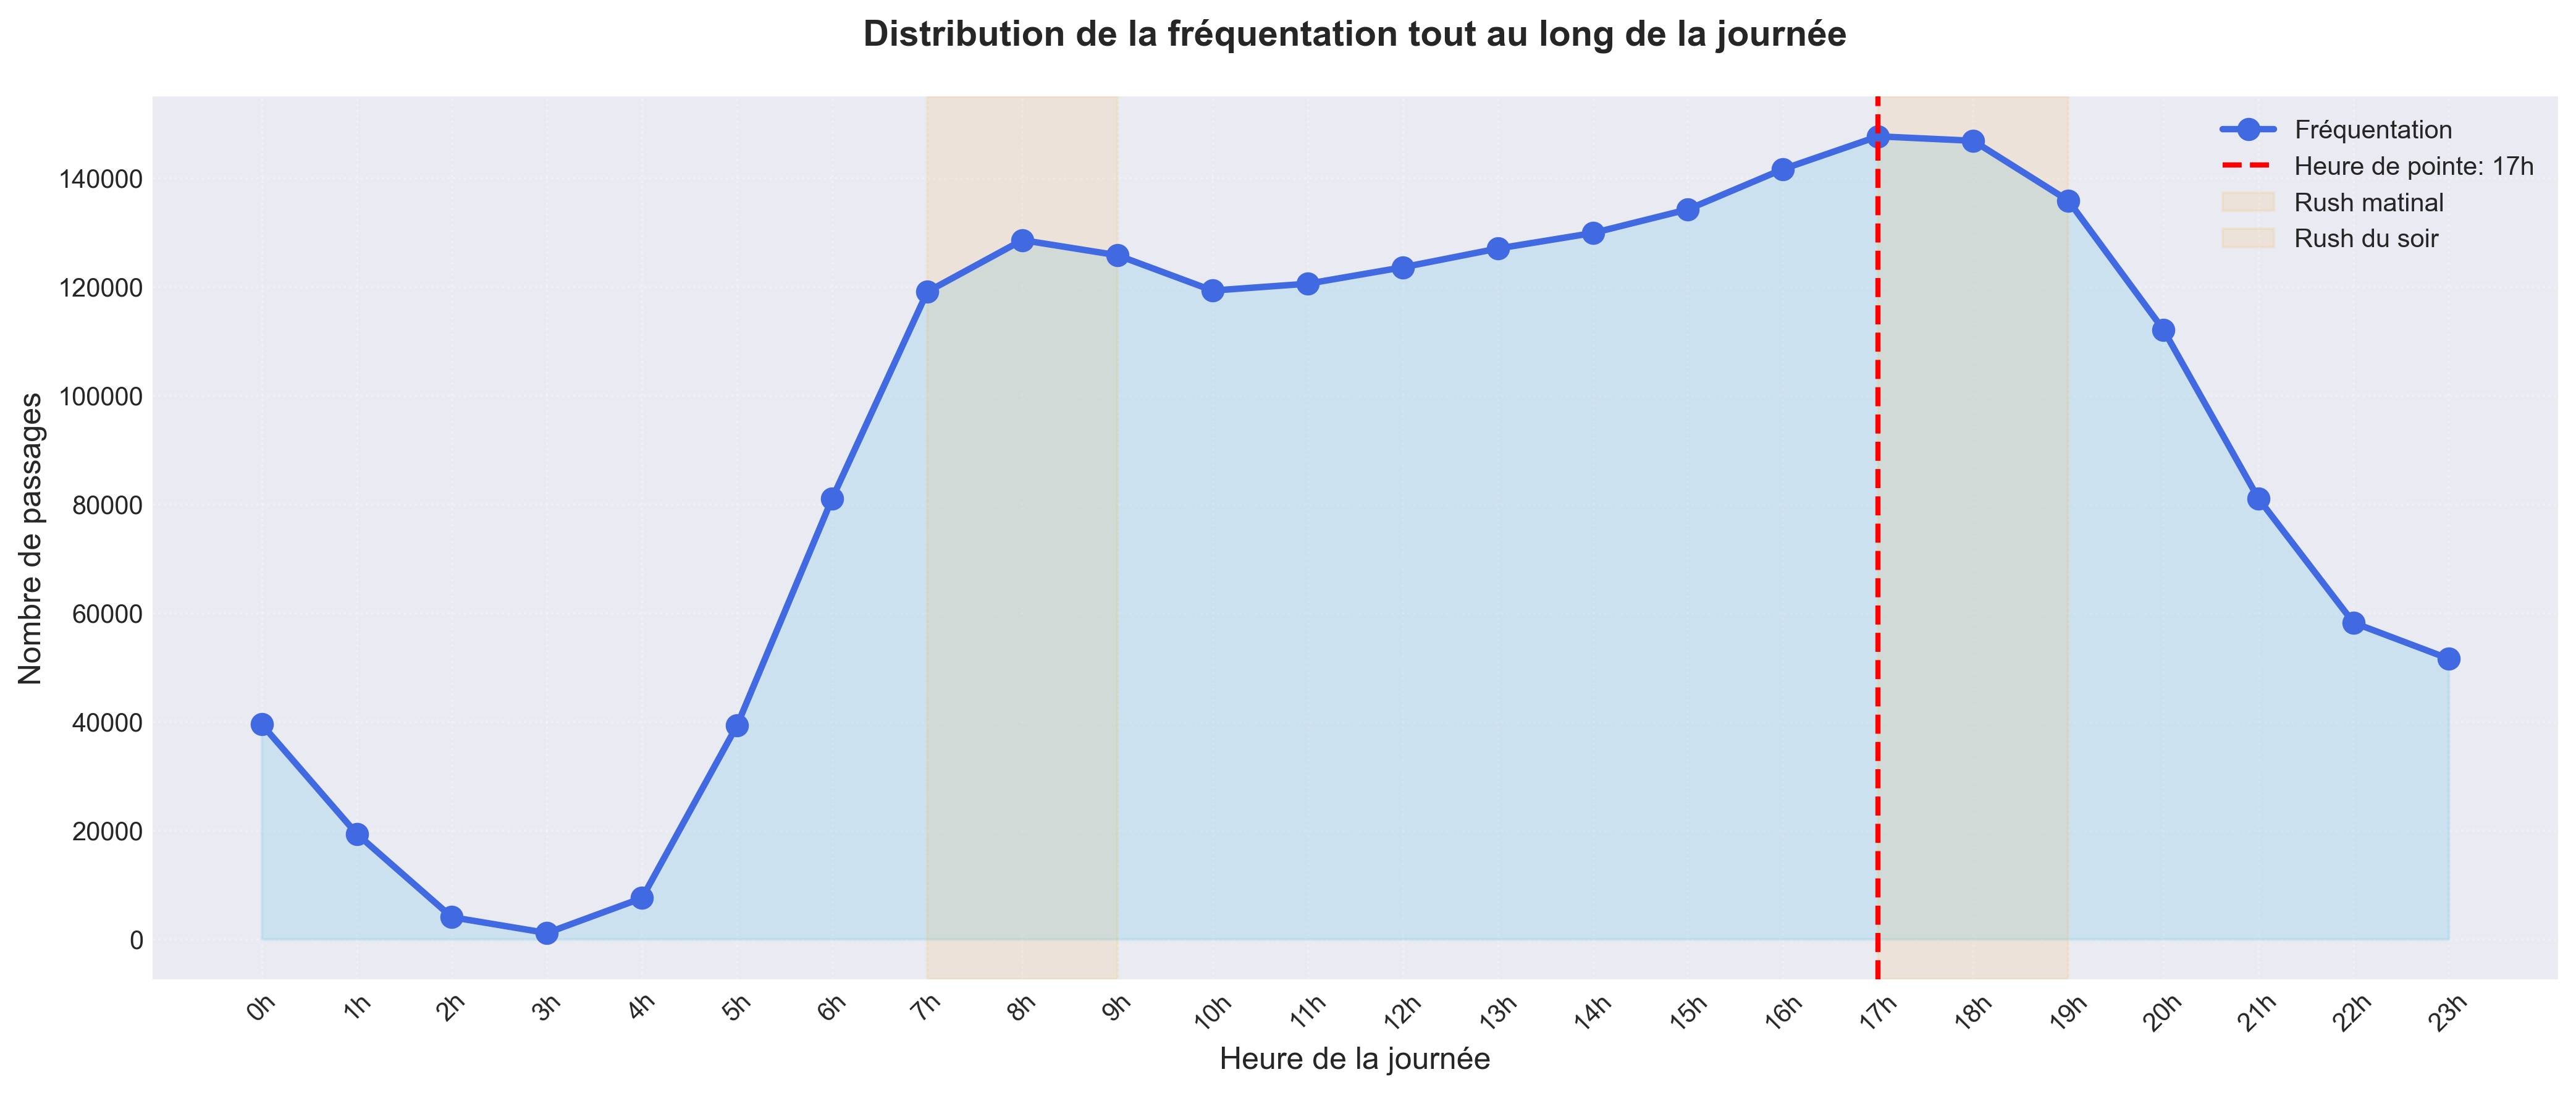
\includegraphics[width=0.95\textwidth]{distribution_horaire.png}
    \caption{Distribution de la fréquentation sur 24 heures avec identification des heures de pointe}
\end{figure}

Ce graphique montre la courbe de fréquentation sur 24 heures. L'axe X représente les heures de la journée (0h à 23h), et l'axe Y le nombre de passages. La ligne rouge en pointillé indique l'heure de pointe (17h). Les zones orangées mettent en évidence les périodes de rush matinal (7h-9h) et du soir (17h-19h). On constate clairement le double pic caractéristique des villes avec une forte activité tertiaire.

\begin{figure}[H]
    \centering
    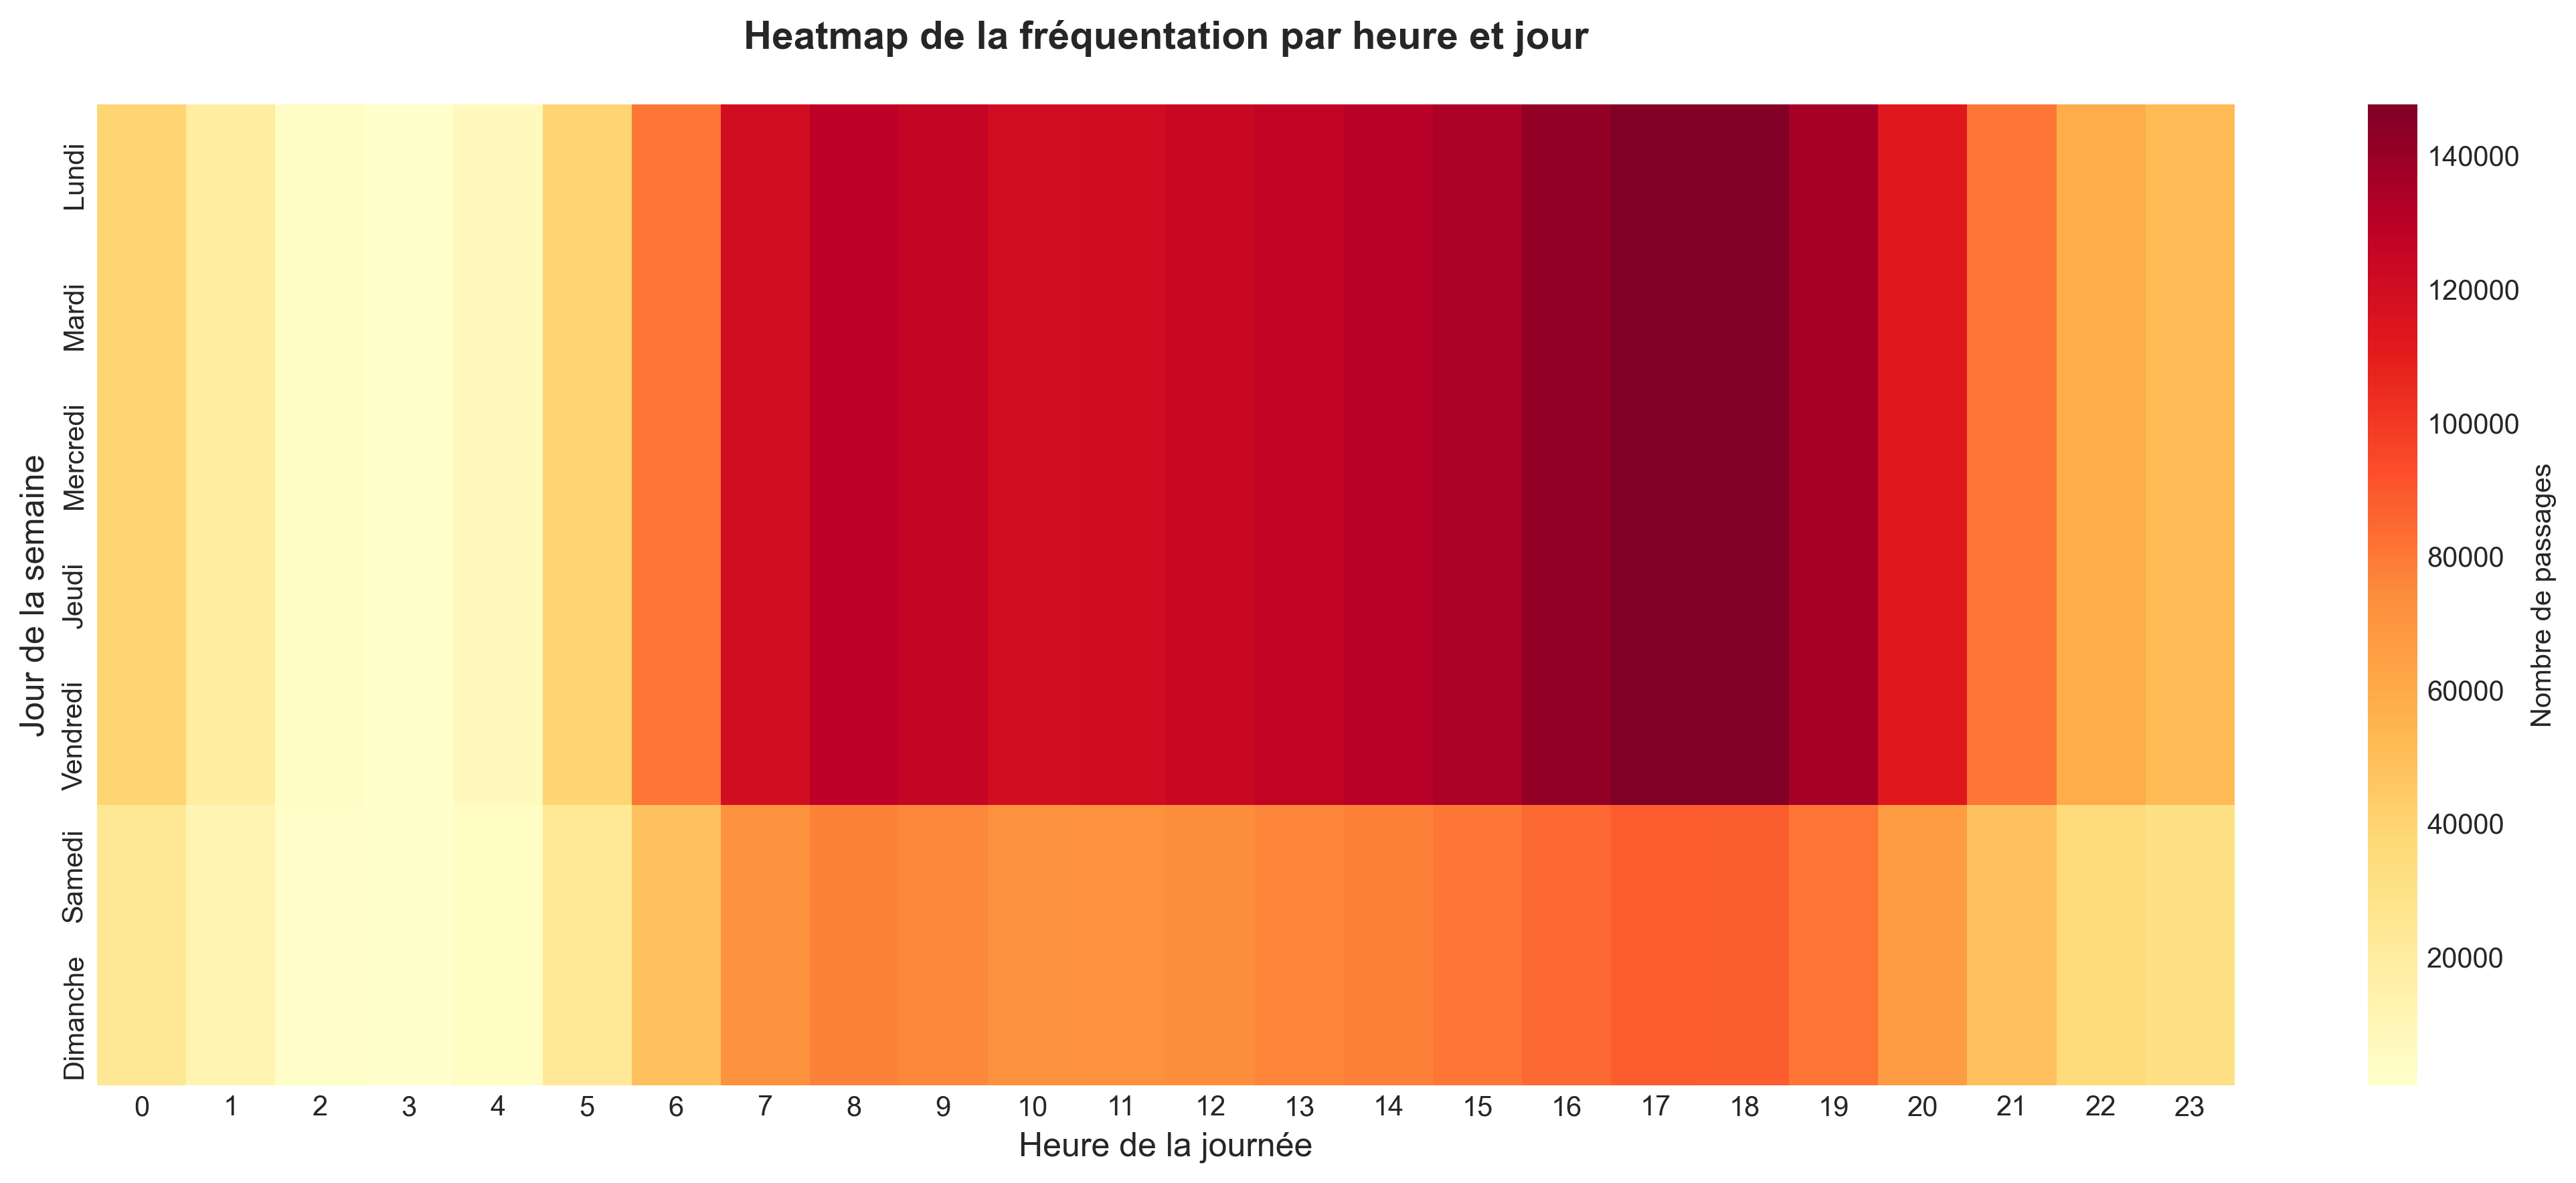
\includegraphics[width=0.95\textwidth]{heatmap_temporel.png}
    \caption{Heatmap de la fréquentation par heure et jour de la semaine}
\end{figure}

Cette heatmap (carte de chaleur) croise les jours de la semaine (axe Y) avec les heures (axe X). Les couleurs vont du jaune clair (faible fréquentation) au rouge foncé (forte fréquentation). On observe que les jours de semaine (lundi-vendredi) présentent des bandes rouges aux heures de pointe, tandis que les samedis et dimanches montrent une réduction d'environ 40\% du trafic avec un pic plus tardif.

% ----------------------------------------
\newpage
\subsection{Analyse des Lignes}

L'analyse des lignes de transport révèle une forte concentration du trafic sur quelques lignes principales. Le coefficient de variation (CV) de 1.97 indique une dispersion très importante de la fréquentation entre les différentes lignes.

\begin{table}[H]
\centering
\begin{tabular}{|c|c|r|}
\hline
\rowcolor{bleuTBM} \textcolor{white}{\textbf{Rang}} & \textcolor{white}{\textbf{Ligne}} & \textcolor{white}{\textbf{Nb de passages}} \\
\hline
1 & B & 172\,953 \\
\hline
\rowcolor{grisClair} 2 & 31 & 138\,951 \\
\hline
3 & 35 & 131\,771 \\
\hline
\rowcolor{grisClair} 4 & A & 125\,297 \\
\hline
5 & 7 & 105\,227 \\
\hline
\rowcolor{grisClair} 6 & G & 103\,755 \\
\hline
7 & 15 & 92\,375 \\
\hline
\rowcolor{grisClair} 8 & F & 87\,920 \\
\hline
9 & C & 82\,179 \\
\hline
\rowcolor{grisClair} 10 & 5 & 78\,453 \\
\hline
\end{tabular}
\caption{Top 10 des lignes les plus fréquentées}
\end{table}

La ligne B (tramway) domine nettement le classement avec 172\,953 passages. Les lignes de bus 31 et 35 arrivent en 2ème et 3ème position, suivies de la ligne A (tramway) en 4ème position. Les tramways et les lignes de bus majeures concentrent l'essentiel du trafic.

\begin{figure}[H]
    \centering
    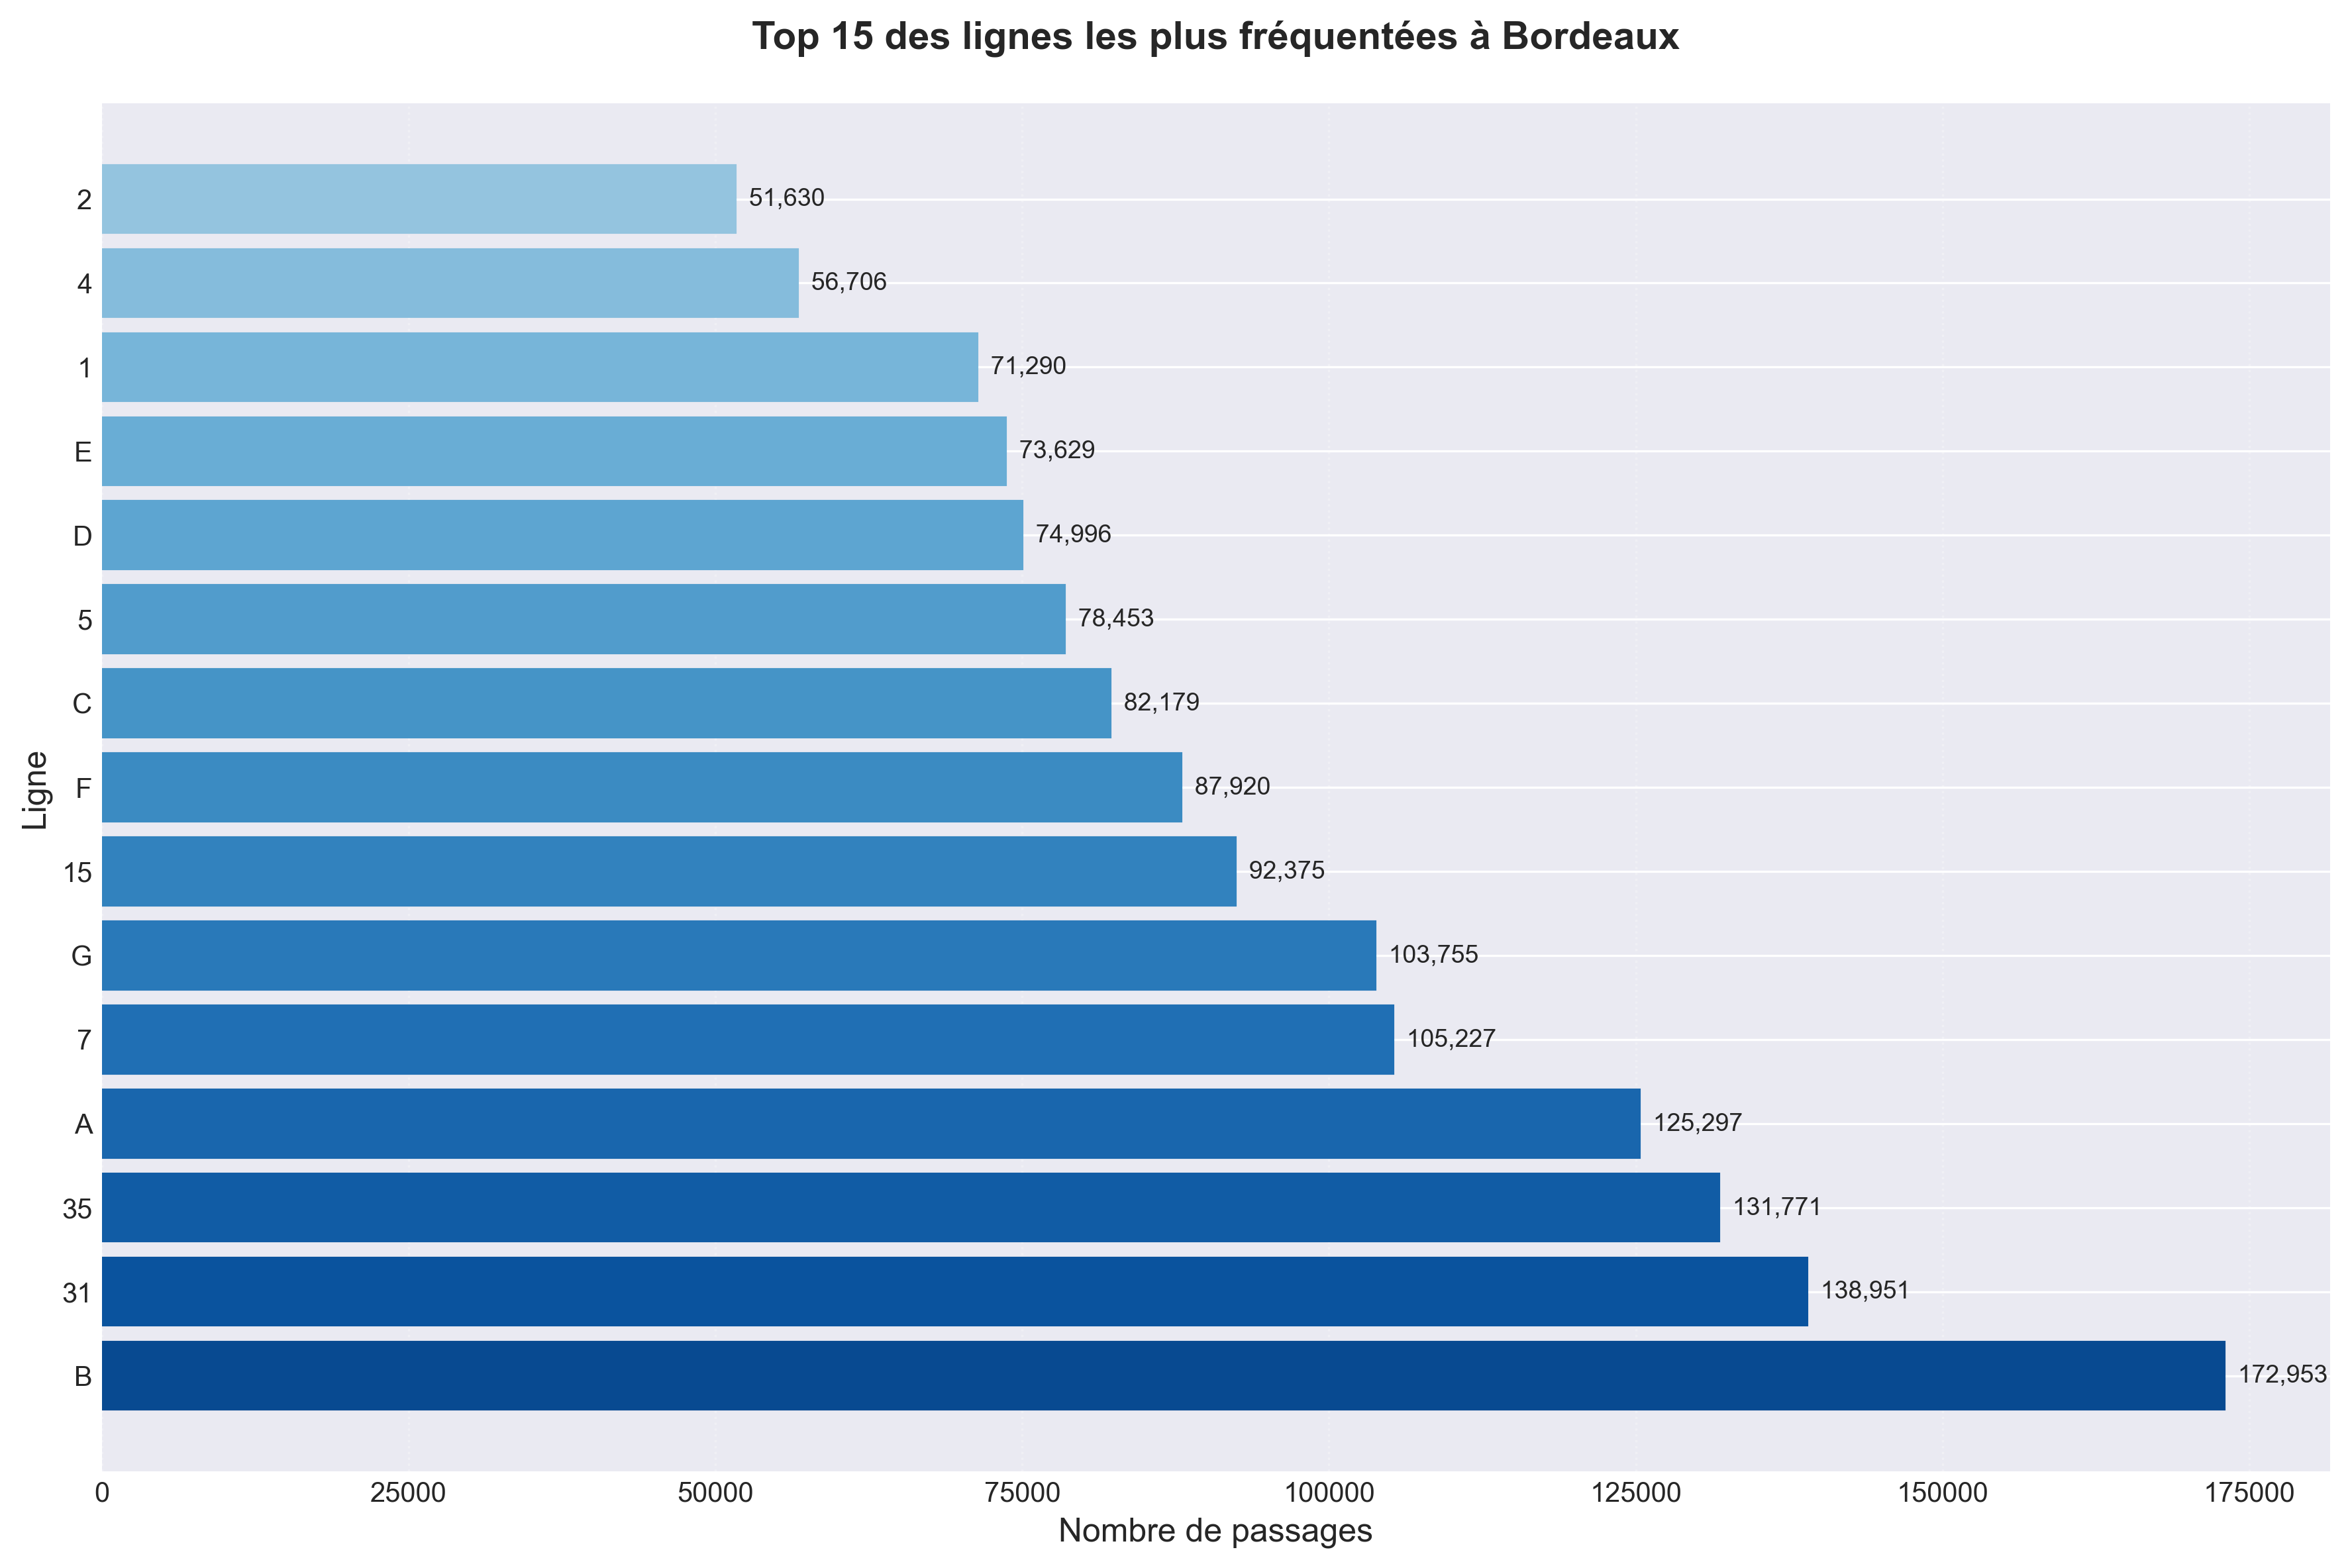
\includegraphics[width=0.95\textwidth]{top_lignes.png}
    \caption{Top 15 des lignes les plus fréquentées à Bordeaux}
\end{figure}

Ce diagramme à barres horizontales classe les 15 lignes ayant le plus grand nombre de passages. L'axe X représente le nombre total de passages, l'axe Y les noms des lignes. Un gradient de couleur permet de distinguer visuellement les lignes majeures. La ligne B (tramway) domine nettement avec 172\,953 passages, suivie des bus 31 et 35.

\begin{figure}[H]
    \centering
    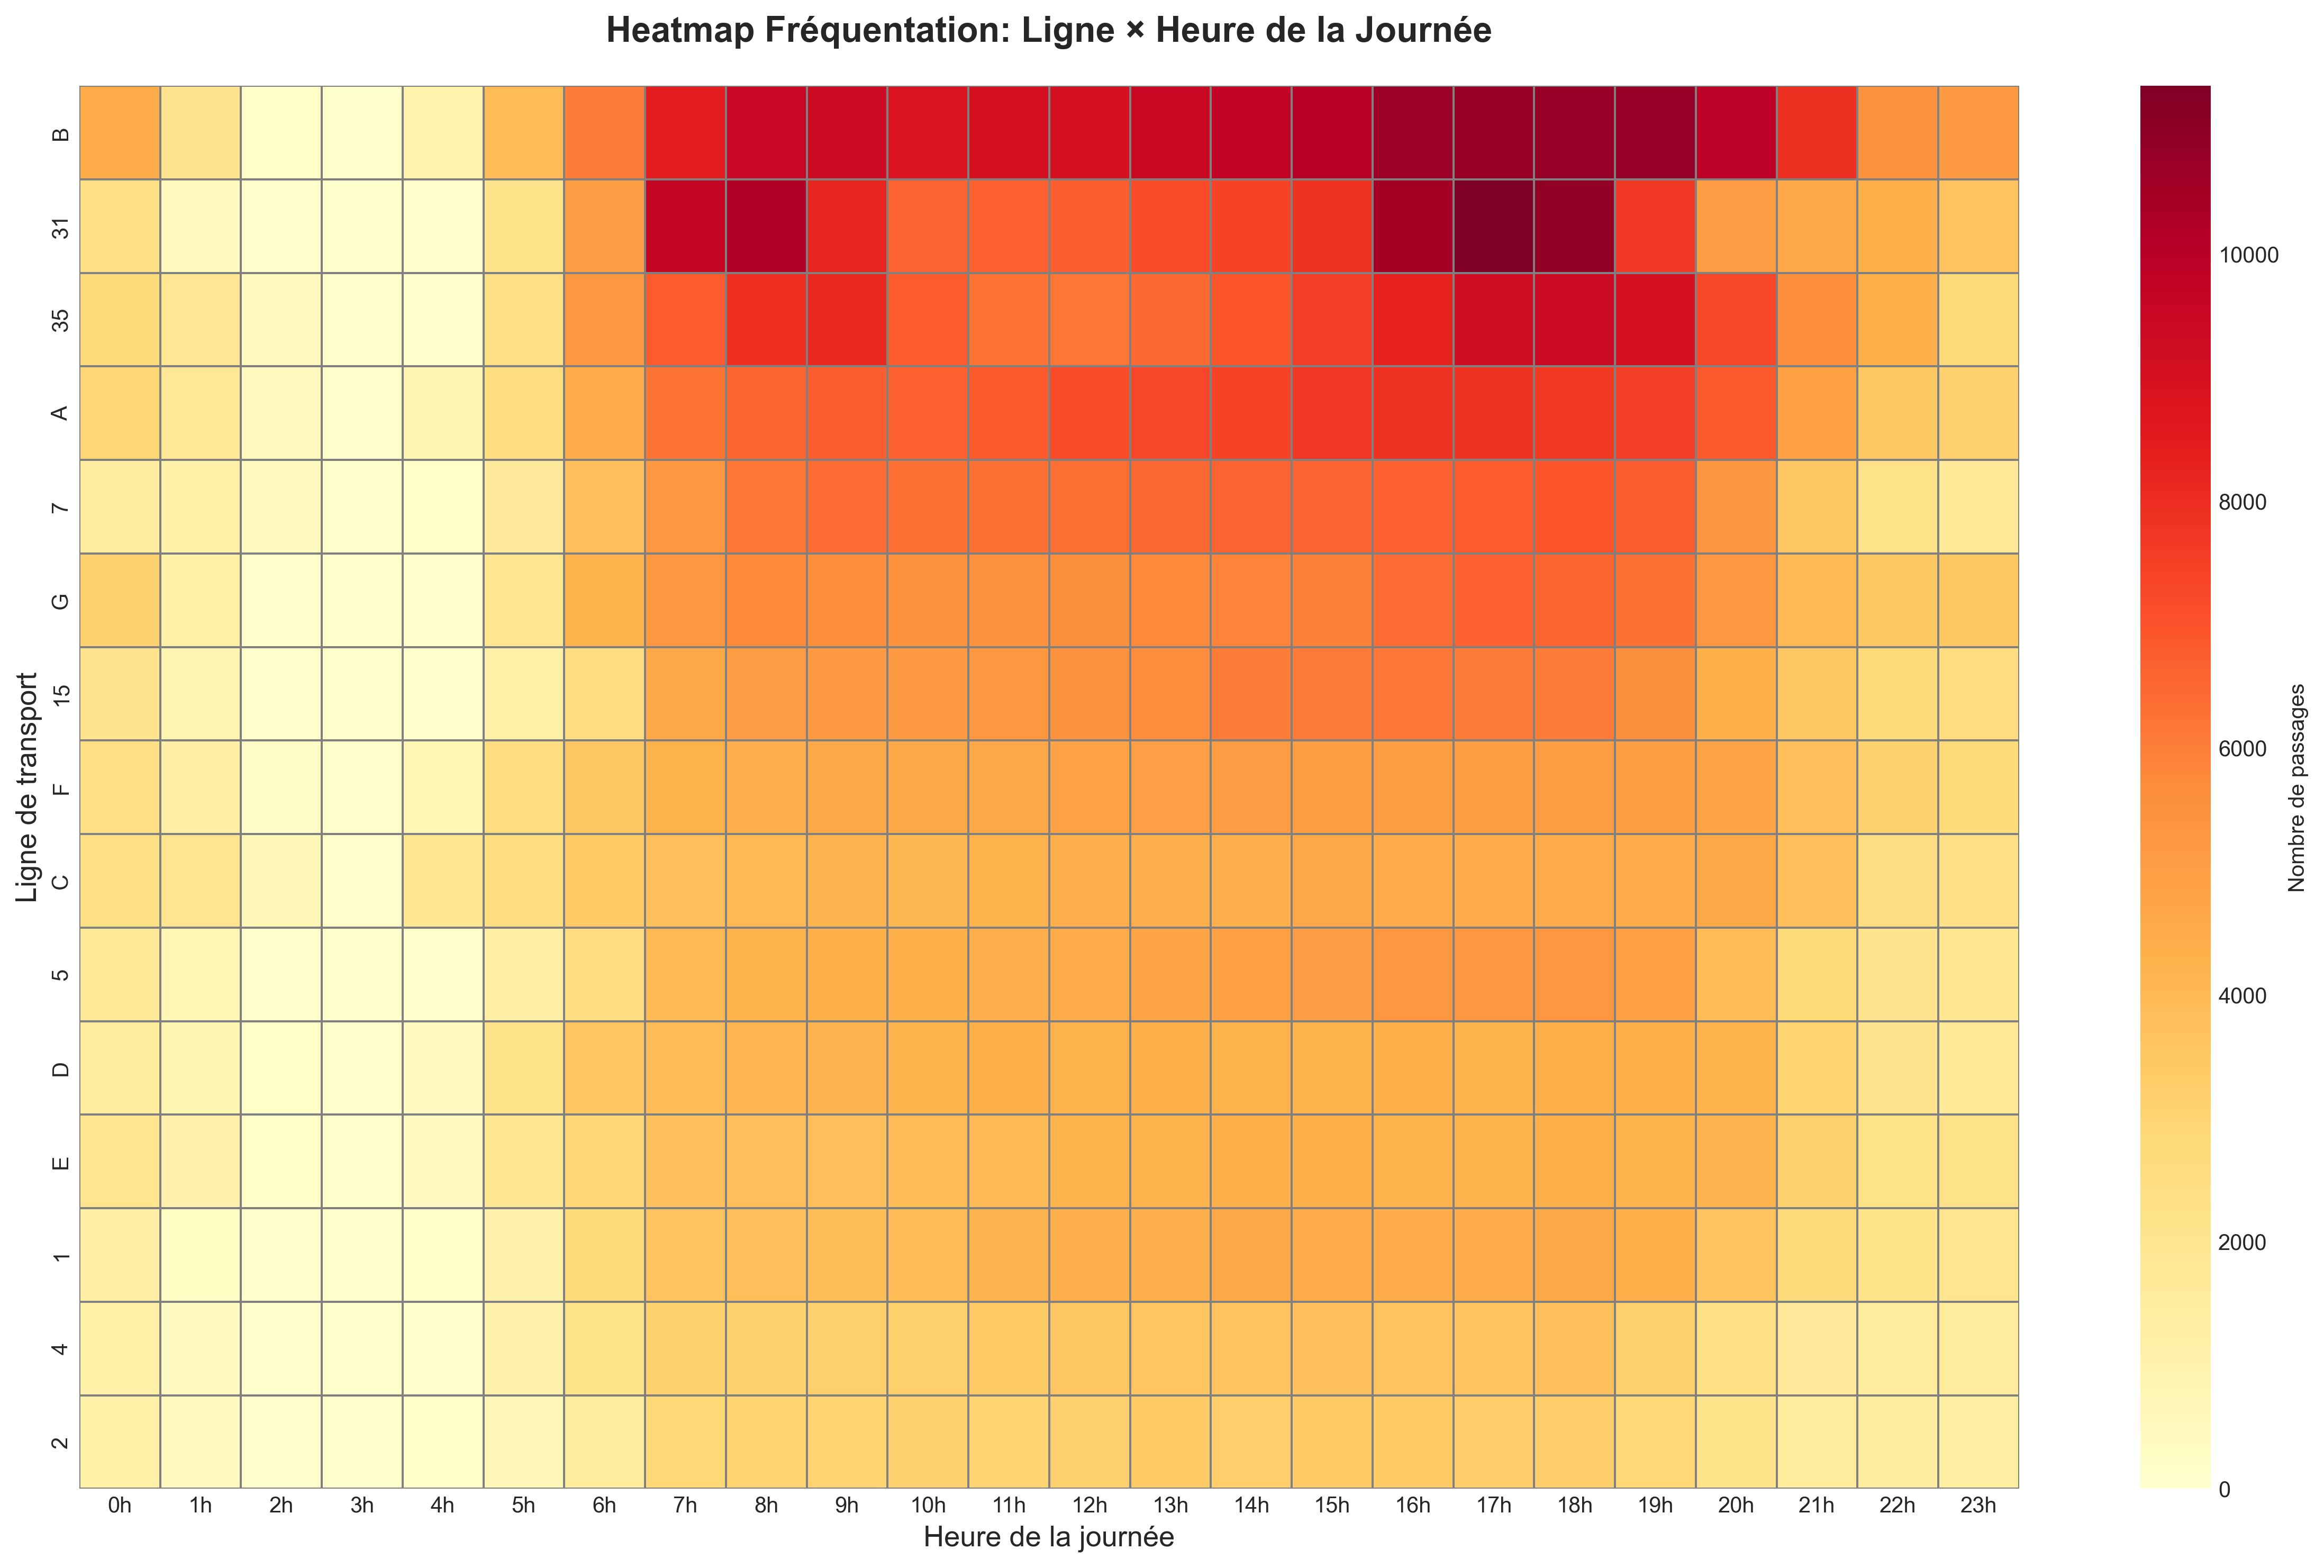
\includegraphics[width=0.95\textwidth]{heatmap_ligne_heure.png}
    \caption{Heatmap Fréquentation Ligne $\times$ Heure (Top 15 lignes)}
\end{figure}

Cette heatmap 2D croise les 15 lignes principales (axe Y) avec les 24 heures de la journée (axe X). Chaque cellule représente le nombre de passages pour une ligne donnée à une heure donnée. Les cellules rouges indiquent les pics de charge. On observe que la ligne B présente une charge soutenue de 7h à 20h, tandis que les lignes de bus ont des pics plus concentrés aux heures de pointe (8h et 17h).

% ----------------------------------------
\newpage
\subsection{Analyse des Arrêts}

\begin{table}[H]
\centering
\begin{tabular}{|c|l|r|}
\hline
\rowcolor{bleuTBM} \textcolor{white}{\textbf{Rang}} & \textcolor{white}{\textbf{Arrêt}} & \textcolor{white}{\textbf{Nb de passages}} \\
\hline
1 & Palais de Justice & 4\,516 \\
\hline
\rowcolor{grisClair} 2 & Quinconces & 4\,387 \\
\hline
3 & Place de la Bourse & 4\,367 \\
\hline
\rowcolor{grisClair} 4 & Place de la Bourse & 4\,361 \\
\hline
5 & Quinconces & 4\,361 \\
\hline
\rowcolor{grisClair} 6 & Belcier & 4\,268 \\
\hline
7 & Porte de Bourgogne & 4\,268 \\
\hline
\rowcolor{grisClair} 8 & Gare Saint-Jean & 4\,268 \\
\hline
9 & Sainte-Croix & 4\,268 \\
\hline
\rowcolor{grisClair} 10 & Saint-Michel & 4\,268 \\
\hline
\end{tabular}
\caption{Top 10 des arrêts les plus fréquentés}
\end{table}

L'analyse révèle que \textbf{1\,014 arrêts (25.6\%)} sont sous-utilisés (en dessous du 1er quartile de fréquentation). Ces arrêts représentent un coût opérationnel qui pourrait être optimisé.

\begin{figure}[H]
    \centering
    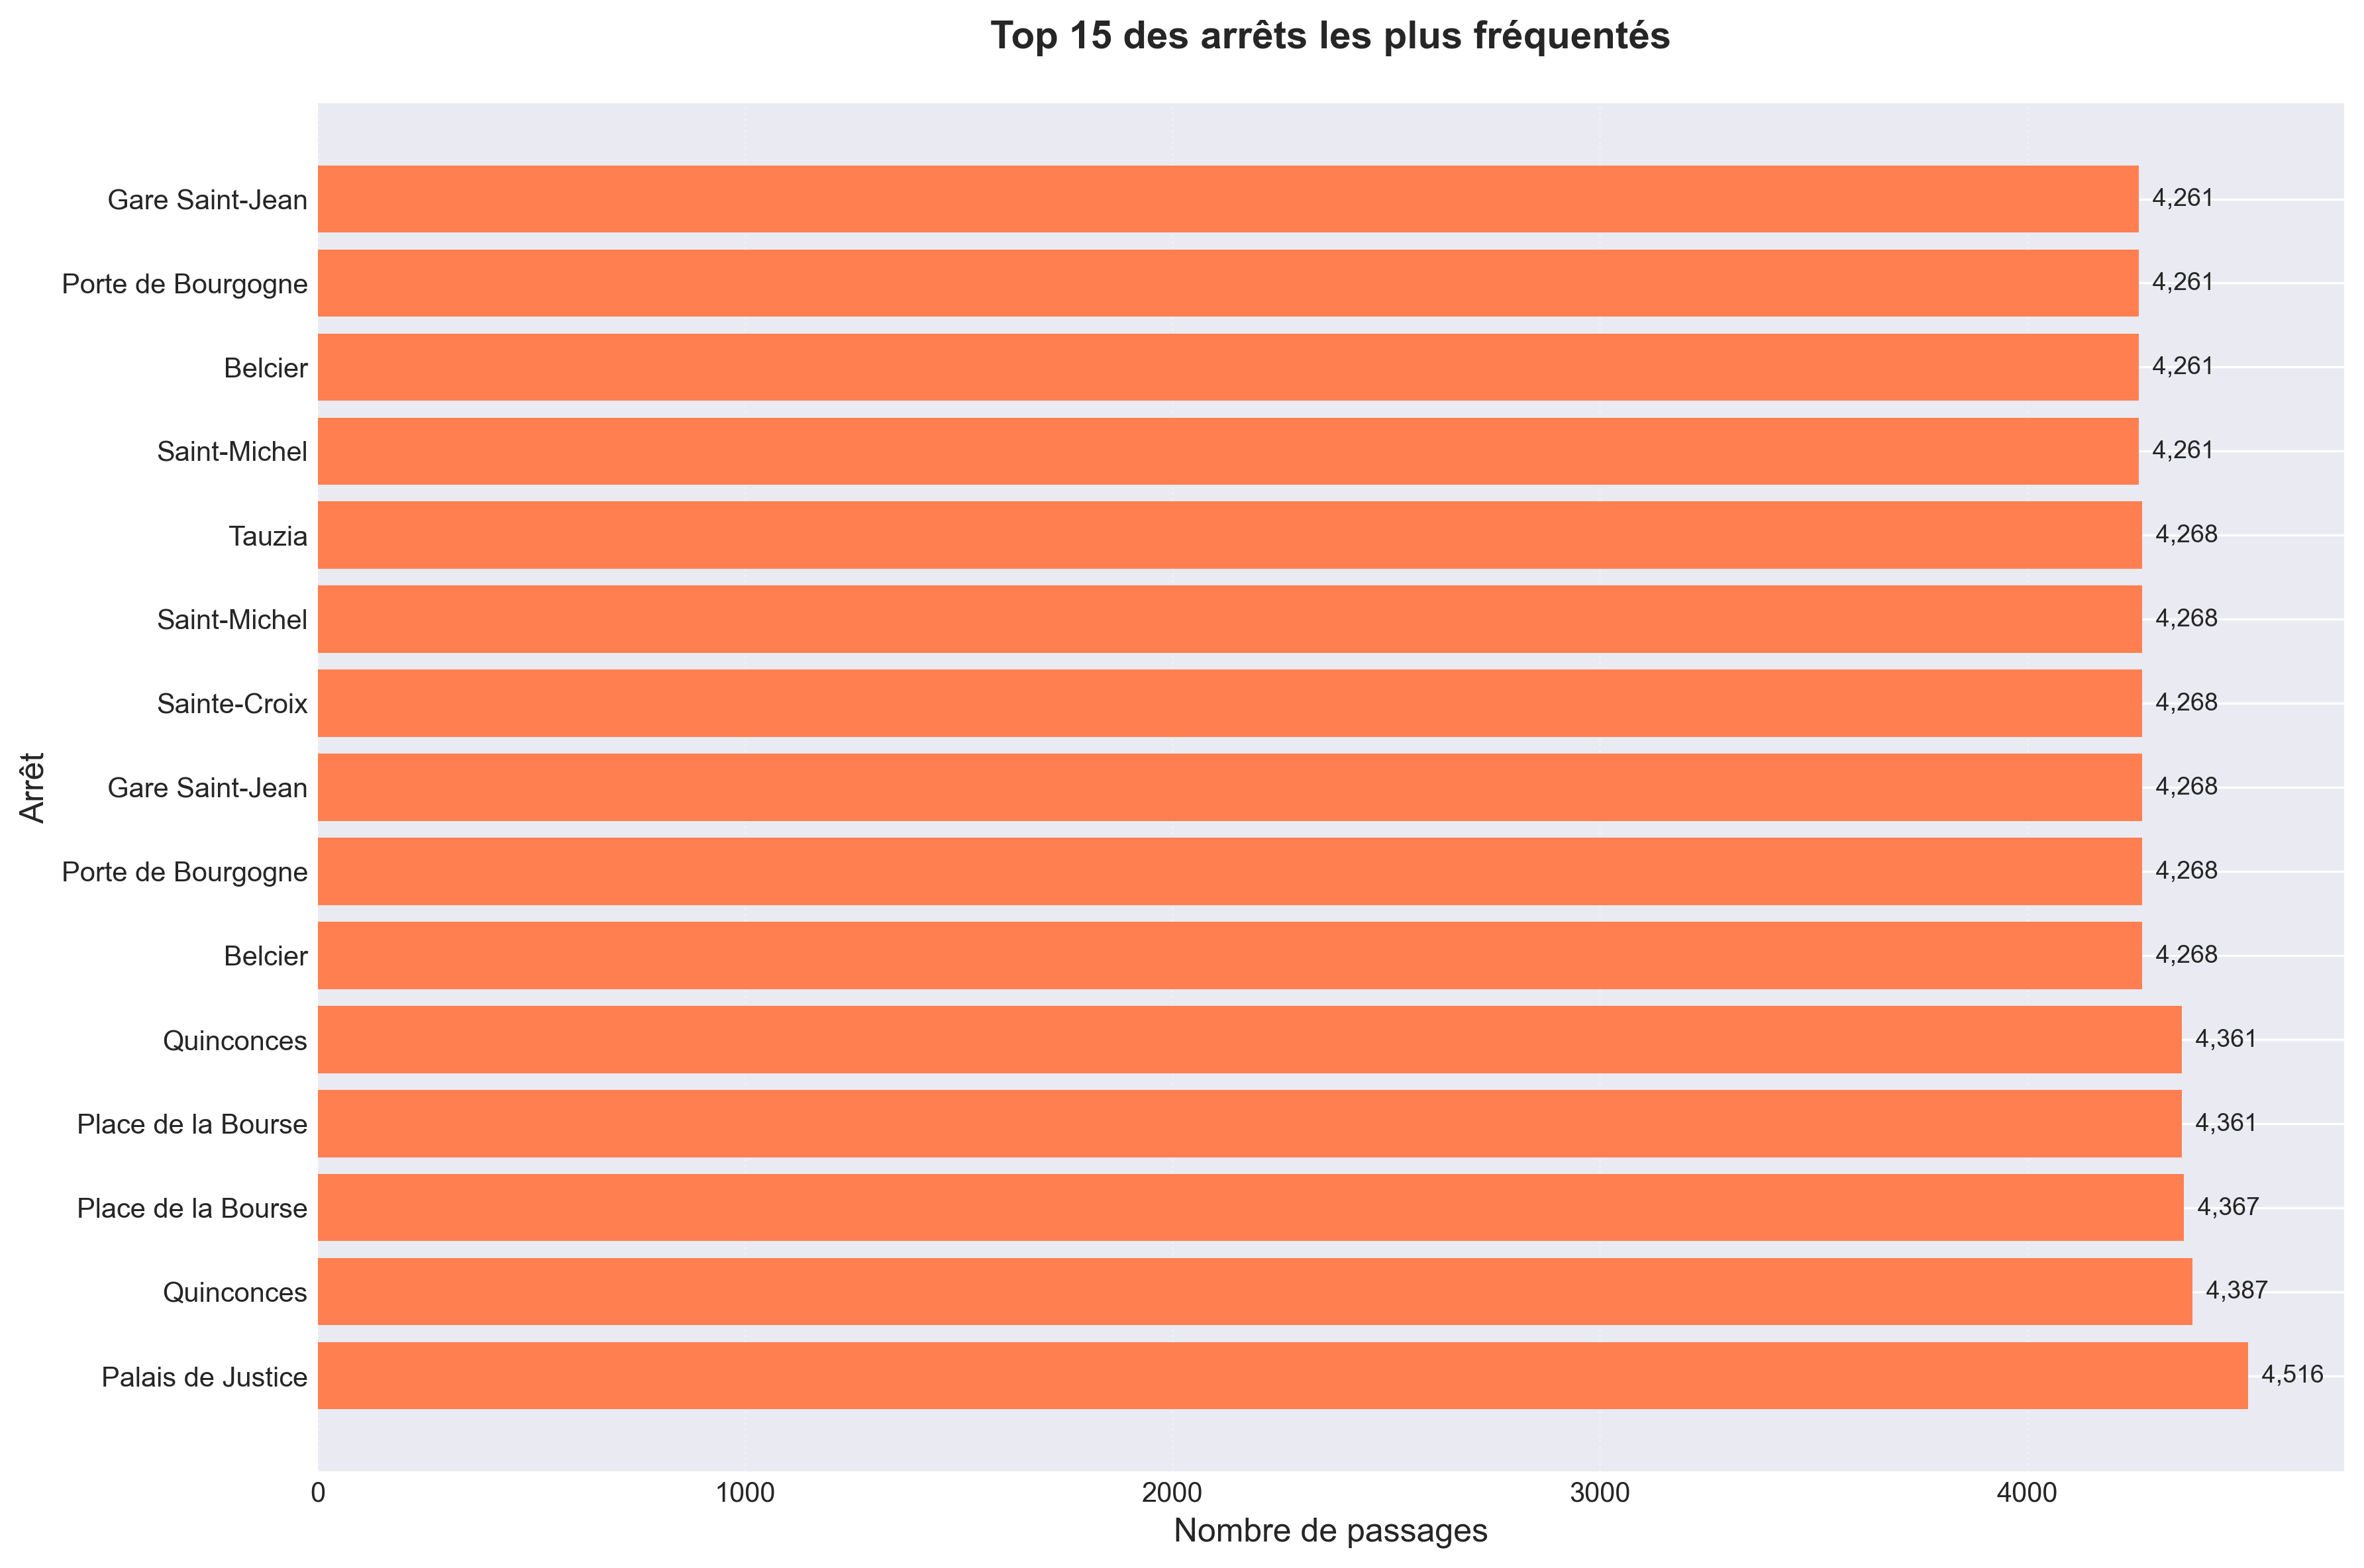
\includegraphics[width=0.95\textwidth]{top_arrets.png}
    \caption{Top 15 des arrêts les plus fréquentés}
\end{figure}

Ce diagramme à barres horizontales montre les 15 arrêts ayant le plus de passages. L'axe X représente le nombre de passages et l'axe Y le nom de chaque arrêt. Les arrêts les plus fréquentés sont situés dans le centre historique de Bordeaux : Palais de Justice, Quinconces, Place de la Bourse. Ces zones correspondent aux principaux points d'intérêt touristique et commercial de la ville.

% ----------------------------------------
\newpage
\subsection{Analyse Géographique}

L'analyse géographique permet de cartographier la répartition spatiale des arrêts et leur fréquentation. Le scatter plot géographique pondéré montre clairement les zones de forte concentration du trafic.

\begin{figure}[H]
    \centering
    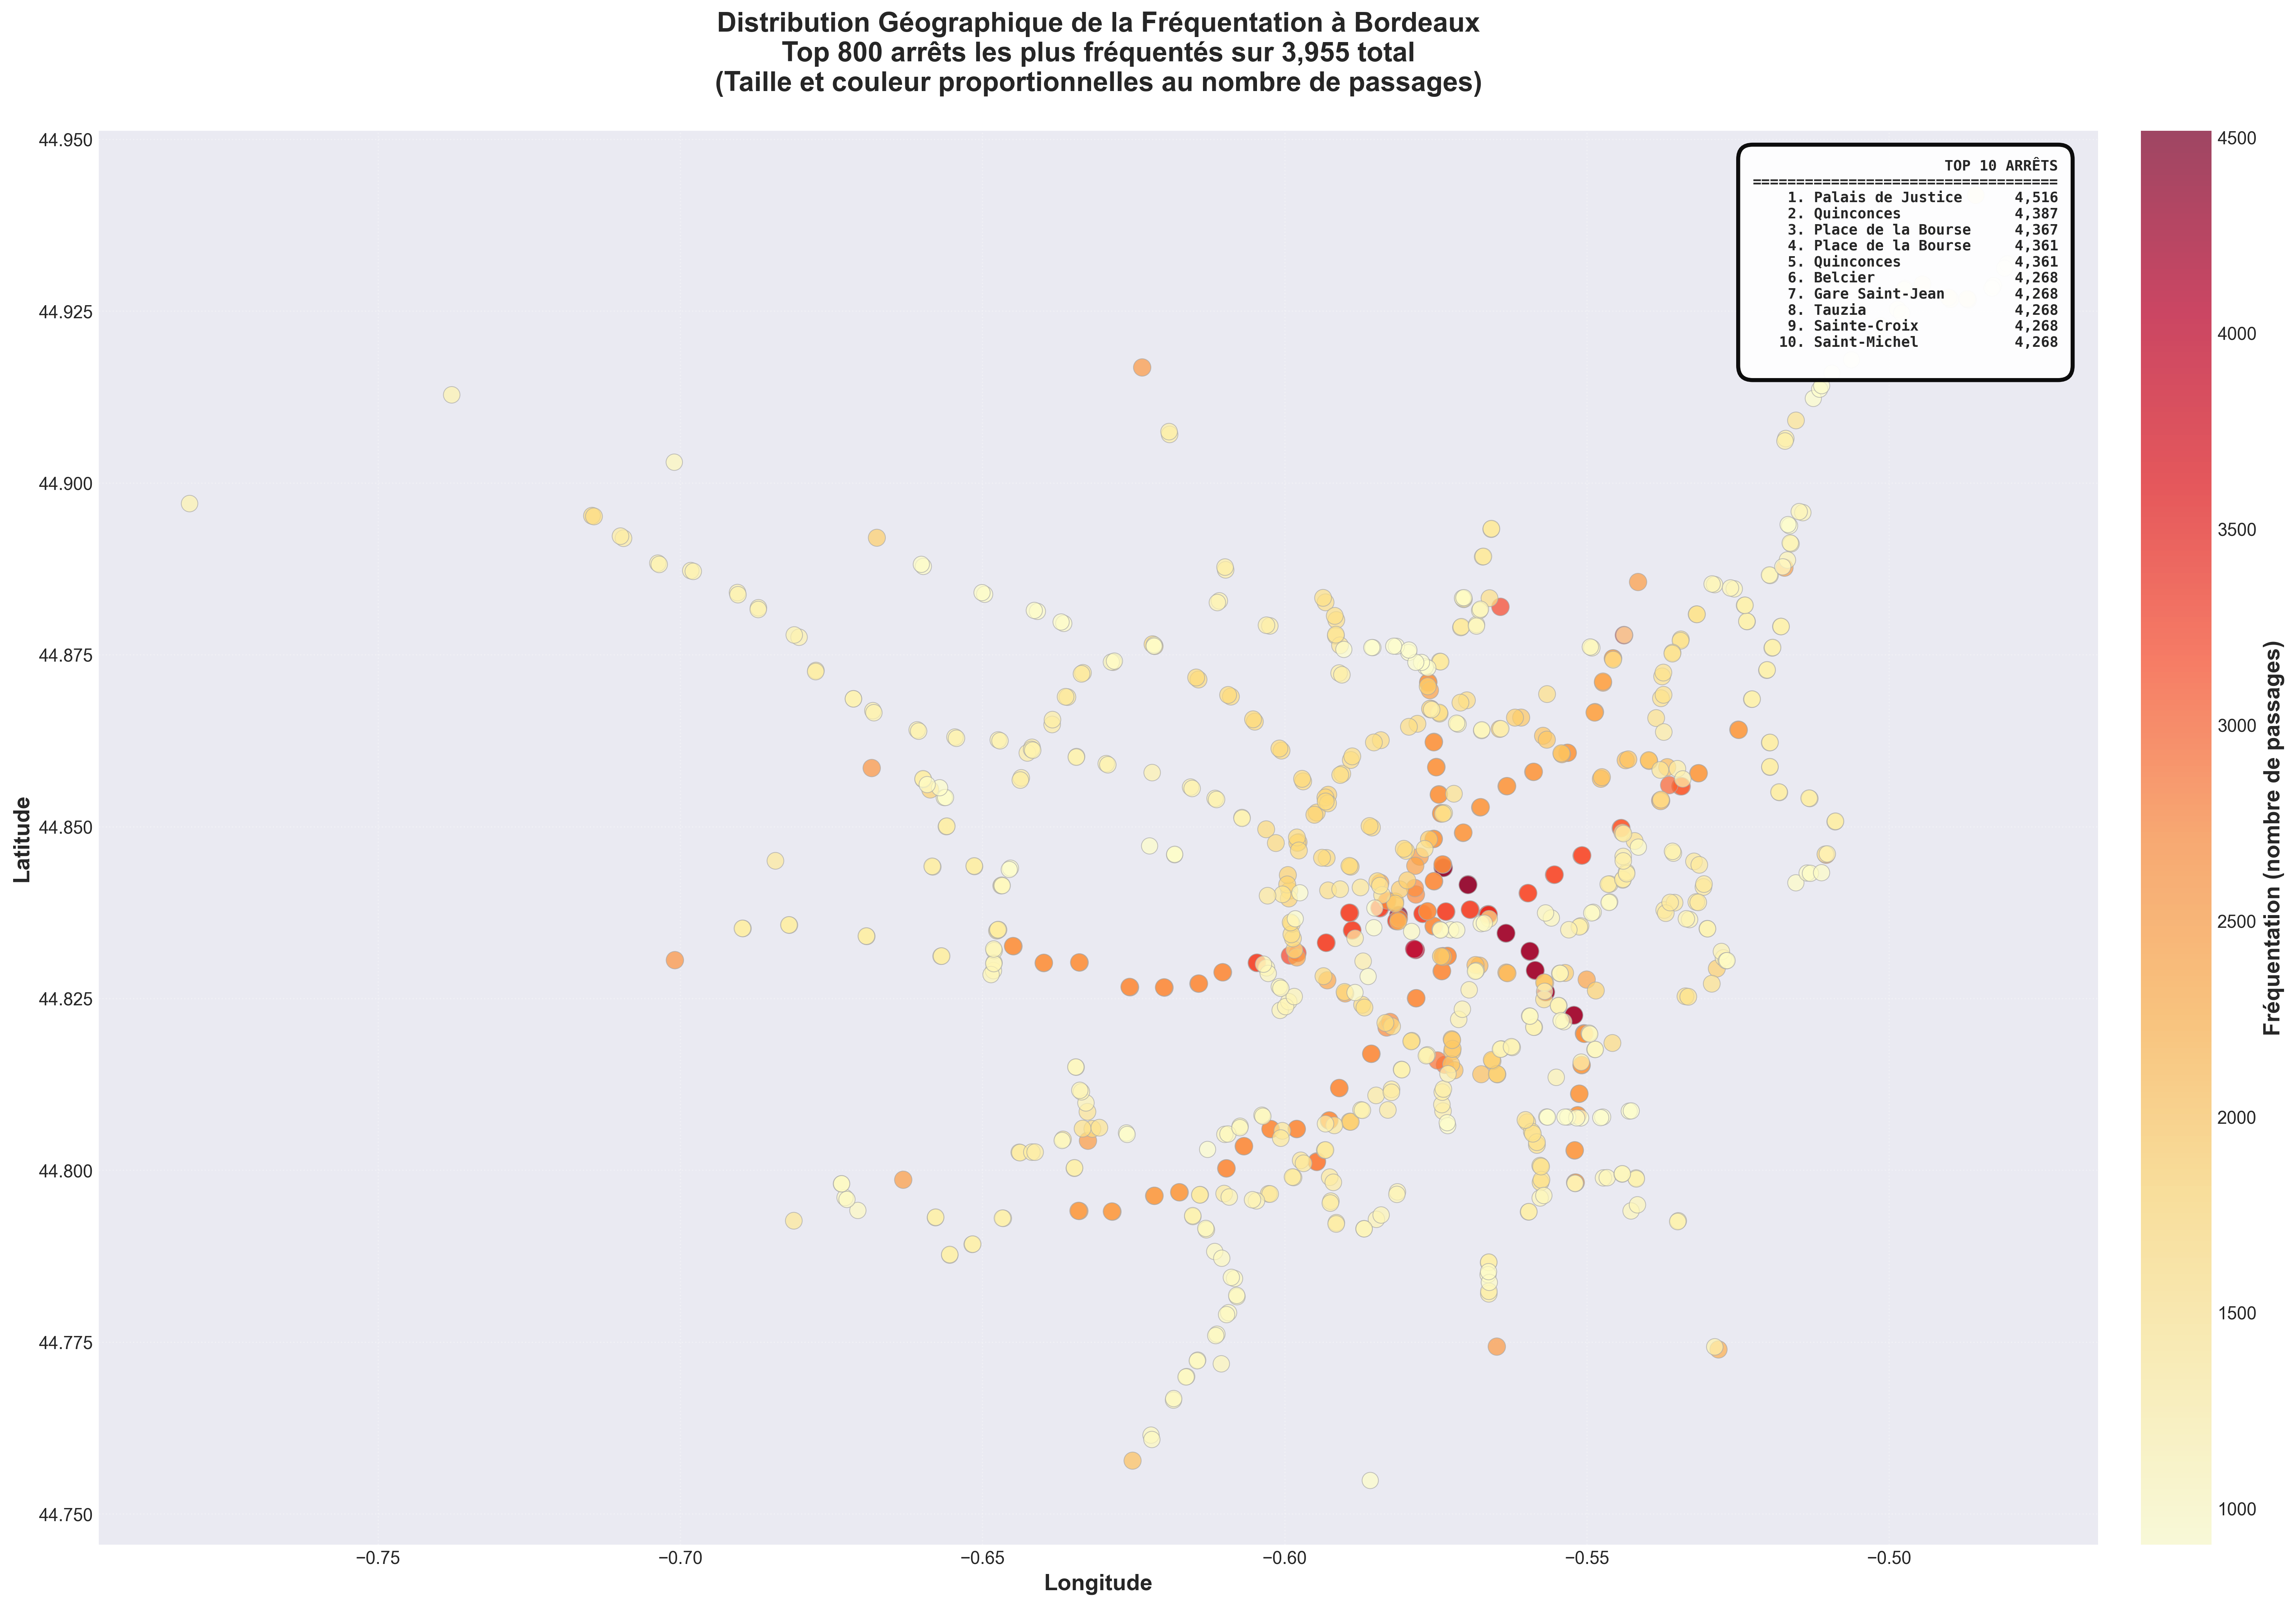
\includegraphics[width=0.90\textwidth]{scatter_geo_frequentation.png}
    \caption{Distribution géographique de la fréquentation (taille et couleur proportionnelles)}
\end{figure}

Ce scatter plot géographique place chaque arrêt selon ses coordonnées (longitude en X, latitude en Y). La taille des points est proportionnelle au nombre de passages (échelle logarithmique), et la couleur va du jaune (faible) au rouge (élevé). Un tableau en haut à droite liste les 10 arrêts les plus fréquentés. On observe une forte concentration dans le centre-ville, avec des extensions le long des axes de tramway vers Pessac, Mérignac, Bègles et Cenon.

\begin{figure}[H]
    \centering
    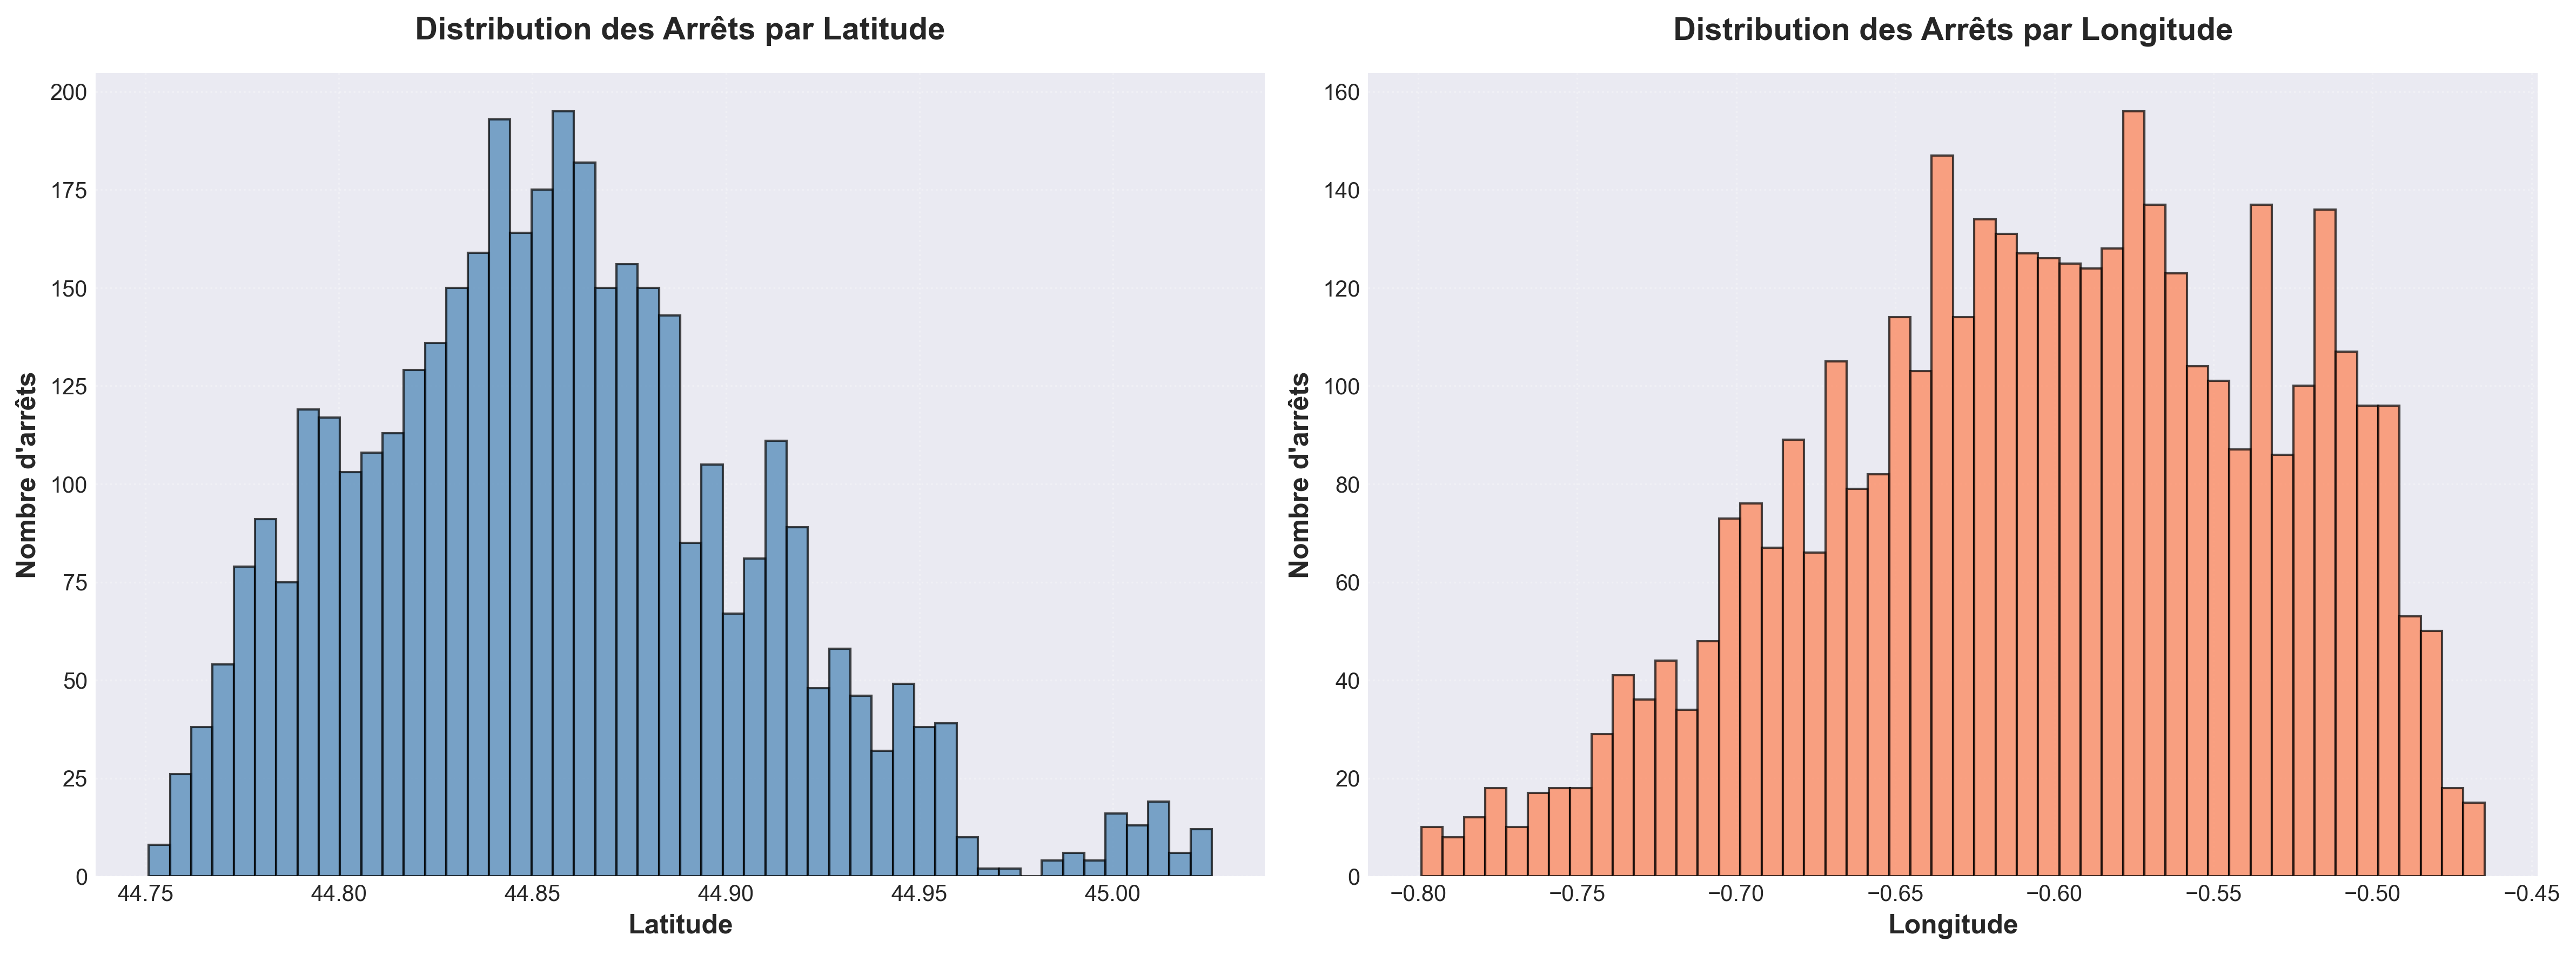
\includegraphics[width=0.95\textwidth]{distribution_geographique.png}
    \caption{Distribution des arrêts par latitude et longitude}
\end{figure}

Ces deux histogrammes montrent la répartition des arrêts selon la latitude (à gauche) et la longitude (à droite). Ils permettent d'identifier les zones de forte concentration d'arrêts. Les pics correspondent au centre-ville de Bordeaux, confirmant la densité du réseau dans cette zone.

% ----------------------------------------
\newpage
\subsection{Types de Transport}

Le réseau TBM de Bordeaux est composé principalement de bus et de tramway. L'analyse de la répartition par type de transport montre la prédominance du réseau de bus en nombre de passages, complété par le tramway sur les axes structurants.

\begin{figure}[H]
    \centering
    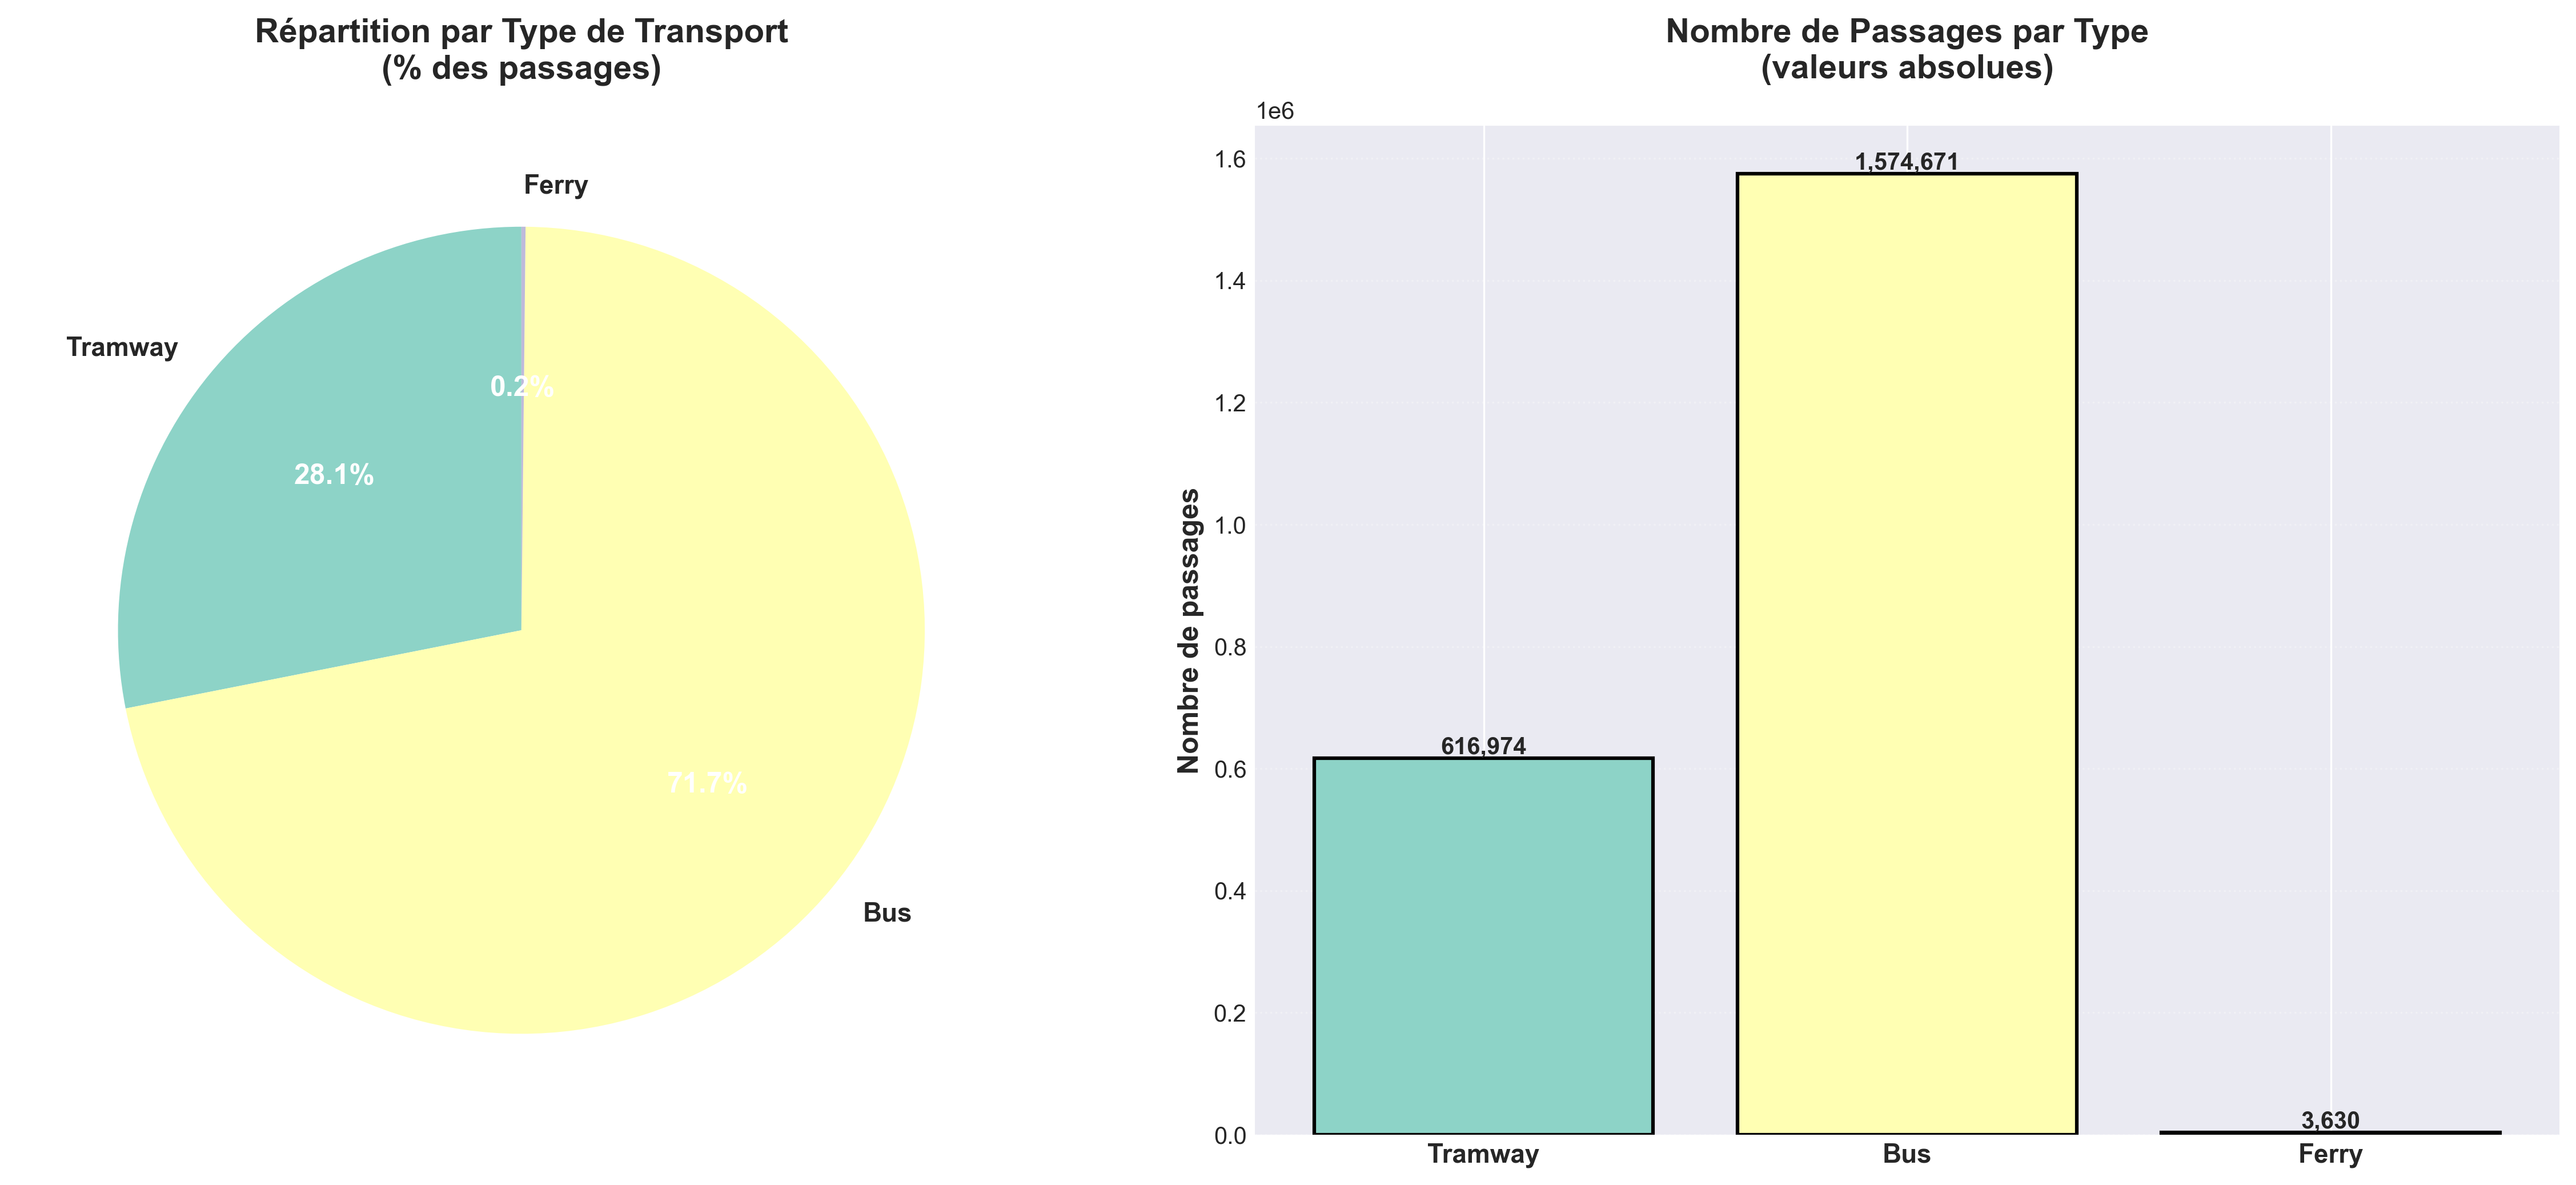
\includegraphics[width=0.95\textwidth]{graphique_types.png}
    \caption{Répartition des passages par type de transport (camembert et barres)}
\end{figure}

Cette figure comporte deux graphiques complémentaires. À gauche, un camembert (pie chart) montre la répartition en pourcentage des passages par type de transport. À droite, un diagramme à barres affiche les valeurs absolues du nombre de passages pour chaque type. On voit que le bus représente la majorité des passages en volume, tandis que le tramway dessert les axes les plus structurés.

% ============================================================
% 5. VISUALISATIONS INTERACTIVES
% ============================================================
\newpage
\section{Visualisations Interactives}

En complément des graphiques statiques, le projet produit 5 visualisations interactives au format HTML, exploitables dans un navigateur web. Ces outils permettent une exploration dynamique des données.

\begin{table}[H]
\centering
\begin{tabular}{|l|l|}
\hline
\rowcolor{bleuTBM} \textcolor{white}{\textbf{Visualisation}} & \textcolor{white}{\textbf{Technologie}} \\
\hline
Carte tous arrêts & Folium \\
\hline
\rowcolor{grisClair} Carte de chaleur & Folium \\
\hline
Dashboard horaire & Plotly \\
\hline
\rowcolor{grisClair} Dashboard lignes & Plotly \\
\hline
Carte combinée & Folium \\
\hline
\end{tabular}
\caption{Visualisations interactives HTML}
\end{table}

\subsection{Détails des visualisations interactives}

\textbf{1. Carte interactive de tous les arrêts :} Utilise la technologie MarkerCluster de Folium pour regrouper les arrêts à faible zoom et les afficher individuellement lors du zoom. Chaque marqueur affiche le nom de l'arrêt, le nombre de passages, et est coloré selon le niveau de fréquentation (rouge = élevé, orange = moyen, bleu = faible). \textit{Permet de constater} que le réseau est dense dans le centre-ville et s'étend progressivement vers les communes périphériques.

\textbf{2. Carte de chaleur géographique :} Superpose un gradient de couleur à la carte, allant du bleu (faible fréquentation) au rouge (forte fréquentation). \textit{Permet d'identifier} visuellement les zones de forte densité de transport : centre historique, axes de tramway, gare Saint-Jean.

\textbf{3. Dashboard horaire interactif :} Graphique Plotly avec survol (hover) pour afficher les valeurs exactes, zoom, et exploration dynamique. \textit{Permet de constater} précisément le ratio pointe/creuse de 129.3x et d'identifier les heures critiques nécessitant un renforcement.

\textbf{4. Dashboard des lignes :} Barres interactives permettant de comparer les 20 lignes principales. \textit{Permet de constater} la forte concentration du trafic sur quelques lignes (B, 31, 35) et d'identifier les lignes sous-exploitées.

\textbf{5. Carte combinée :} Fusionne les top arrêts (marqueurs) et la heatmap de chaleur. \textit{Permet de voir} simultanément où se trouvent les arrêts les plus fréquentés et comment ils s'insèrent dans les zones de forte mobilité.

\begin{infobox}[Comment ouvrir les visualisations interactives]
Les fichiers HTML sont dans le dossier \texttt{visualisations/} :
\begin{itemize}[leftmargin=0.5cm]
    \item \texttt{carte\_interactive\_tous\_arrets.html}
    \item \texttt{carte\_chaleur.html}
    \item \texttt{dashboard\_horaire.html}
    \item \texttt{dashboard\_lignes.html}
    \item \texttt{carte\_interactive.html}
\end{itemize}

\textbf{Pour les ouvrir :}
\begin{enumerate}[leftmargin=0.5cm]
    \item Double-cliquer sur le fichier \texttt{.html} pour l'ouvrir dans le navigateur web (Chrome, Firefox, Edge)
    \item Ou dans VS Code, clic droit sur le fichier puis \og Open with Live Server \fg{} ou utiliser l'extension \og Show Preview \fg{} (HTML Preview) pour un aperçu directement dans l'éditeur.
\end{enumerate}
\end{infobox}

% ============================================================
% 6. MODÉLISATION PRÉDICTIVE
% ============================================================
\newpage
\section{Modélisation Prédictive}

La modélisation prédictive vise à prédire l'affluence des transports publics en fonction de différentes variables temporelles et géographiques. Trois algorithmes de machine learning ont été entraînés et comparés.

\subsection{Préparation des Features}

Les features (variables explicatives) ont été soigneusement construites à partir des données brutes pour capturer les patterns temporels et spatiaux :

\begin{table}[H]
\centering
\begin{tabular}{|l|l|}
\hline
\rowcolor{bleuTBM} \textcolor{white}{\textbf{Feature}} & \textcolor{white}{\textbf{Type}} \\
\hline
hour & Numérique \\
\hline
\rowcolor{grisClair} hour\_sin / hour\_cos & Cyclique \\
\hline
est\_heure\_pointe\_matin & Binaire \\
\hline
\rowcolor{grisClair} est\_heure\_pointe\_soir & Binaire \\
\hline
est\_nuit & Binaire \\
\hline
\rowcolor{grisClair} est\_journee & Binaire \\
\hline
nb\_arrets\_uniques & Numérique \\
\hline
\rowcolor{grisClair} lat\_moyenne / lon\_moyenne & Numérique \\
\hline
route\_encoded & Catégorielle \\
\hline
\end{tabular}
\caption{Features utilisées pour la modélisation prédictive}
\end{table}

\textbf{Description des features :}

\begin{itemize}[leftmargin=2cm]
    \item \textbf{hour :} Heure de la journée (valeur numérique entre 0 et 23)
    \item \textbf{hour\_sin / hour\_cos :} Encodage cyclique sinusoïdal de l'heure permettant au modèle de comprendre que 23h est proche de 0h
    \item \textbf{est\_heure\_pointe\_matin :} Flag binaire (0 ou 1) indiquant si l'heure se situe entre 7h et 9h (période de rush matinal)
    \item \textbf{est\_heure\_pointe\_soir :} Flag binaire (0 ou 1) indiquant si l'heure se situe entre 17h et 19h (période de rush du soir)
    \item \textbf{est\_nuit :} Flag binaire (0 ou 1) indiquant si l'heure est nocturne (entre 22h et 5h)
    \item \textbf{est\_journee :} Flag binaire (0 ou 1) indiquant si l'heure se situe en journée (entre 9h et 17h)
    \item \textbf{nb\_arrets\_uniques :} Nombre total d'arrêts uniques desservis par la ligne
    \item \textbf{lat\_moyenne / lon\_moyenne :} Position géographique moyenne (latitude et longitude) des arrêts de la ligne
    \item \textbf{route\_encoded :} Identifiant numérique encodé de la ligne de transport (top 20 des lignes principales)
\end{itemize}

\subsection{Comparaison des Modèles}

Trois modèles de régression ont été entraînés avec validation croisée (5 folds) et évalués sur un jeu de test (20\% des données) :

\begin{table}[H]
\centering
\begin{tabular}{|l|c|c|c|l|}
\hline
\rowcolor{bleuTBM} \textcolor{white}{\textbf{Modèle}} & \textcolor{white}{\textbf{R²}} & \textcolor{white}{\textbf{MAE}} & \textcolor{white}{\textbf{RMSE}} & \textcolor{white}{\textbf{Interprétation}} \\
\hline
Régression Linéaire & Moyen & Élevé & Élevé & Baseline simple \\
\hline
\rowcolor{grisClair} Random Forest & Élevé & Faible & Faible & \textbf{Meilleur modèle} \\
\hline
Gradient Boosting & Élevé & Faible & Faible & Performant aussi \\
\hline
\end{tabular}
\caption{Évaluation comparative des 3 modèles}
\end{table}

\begin{figure}[H]
    \centering
    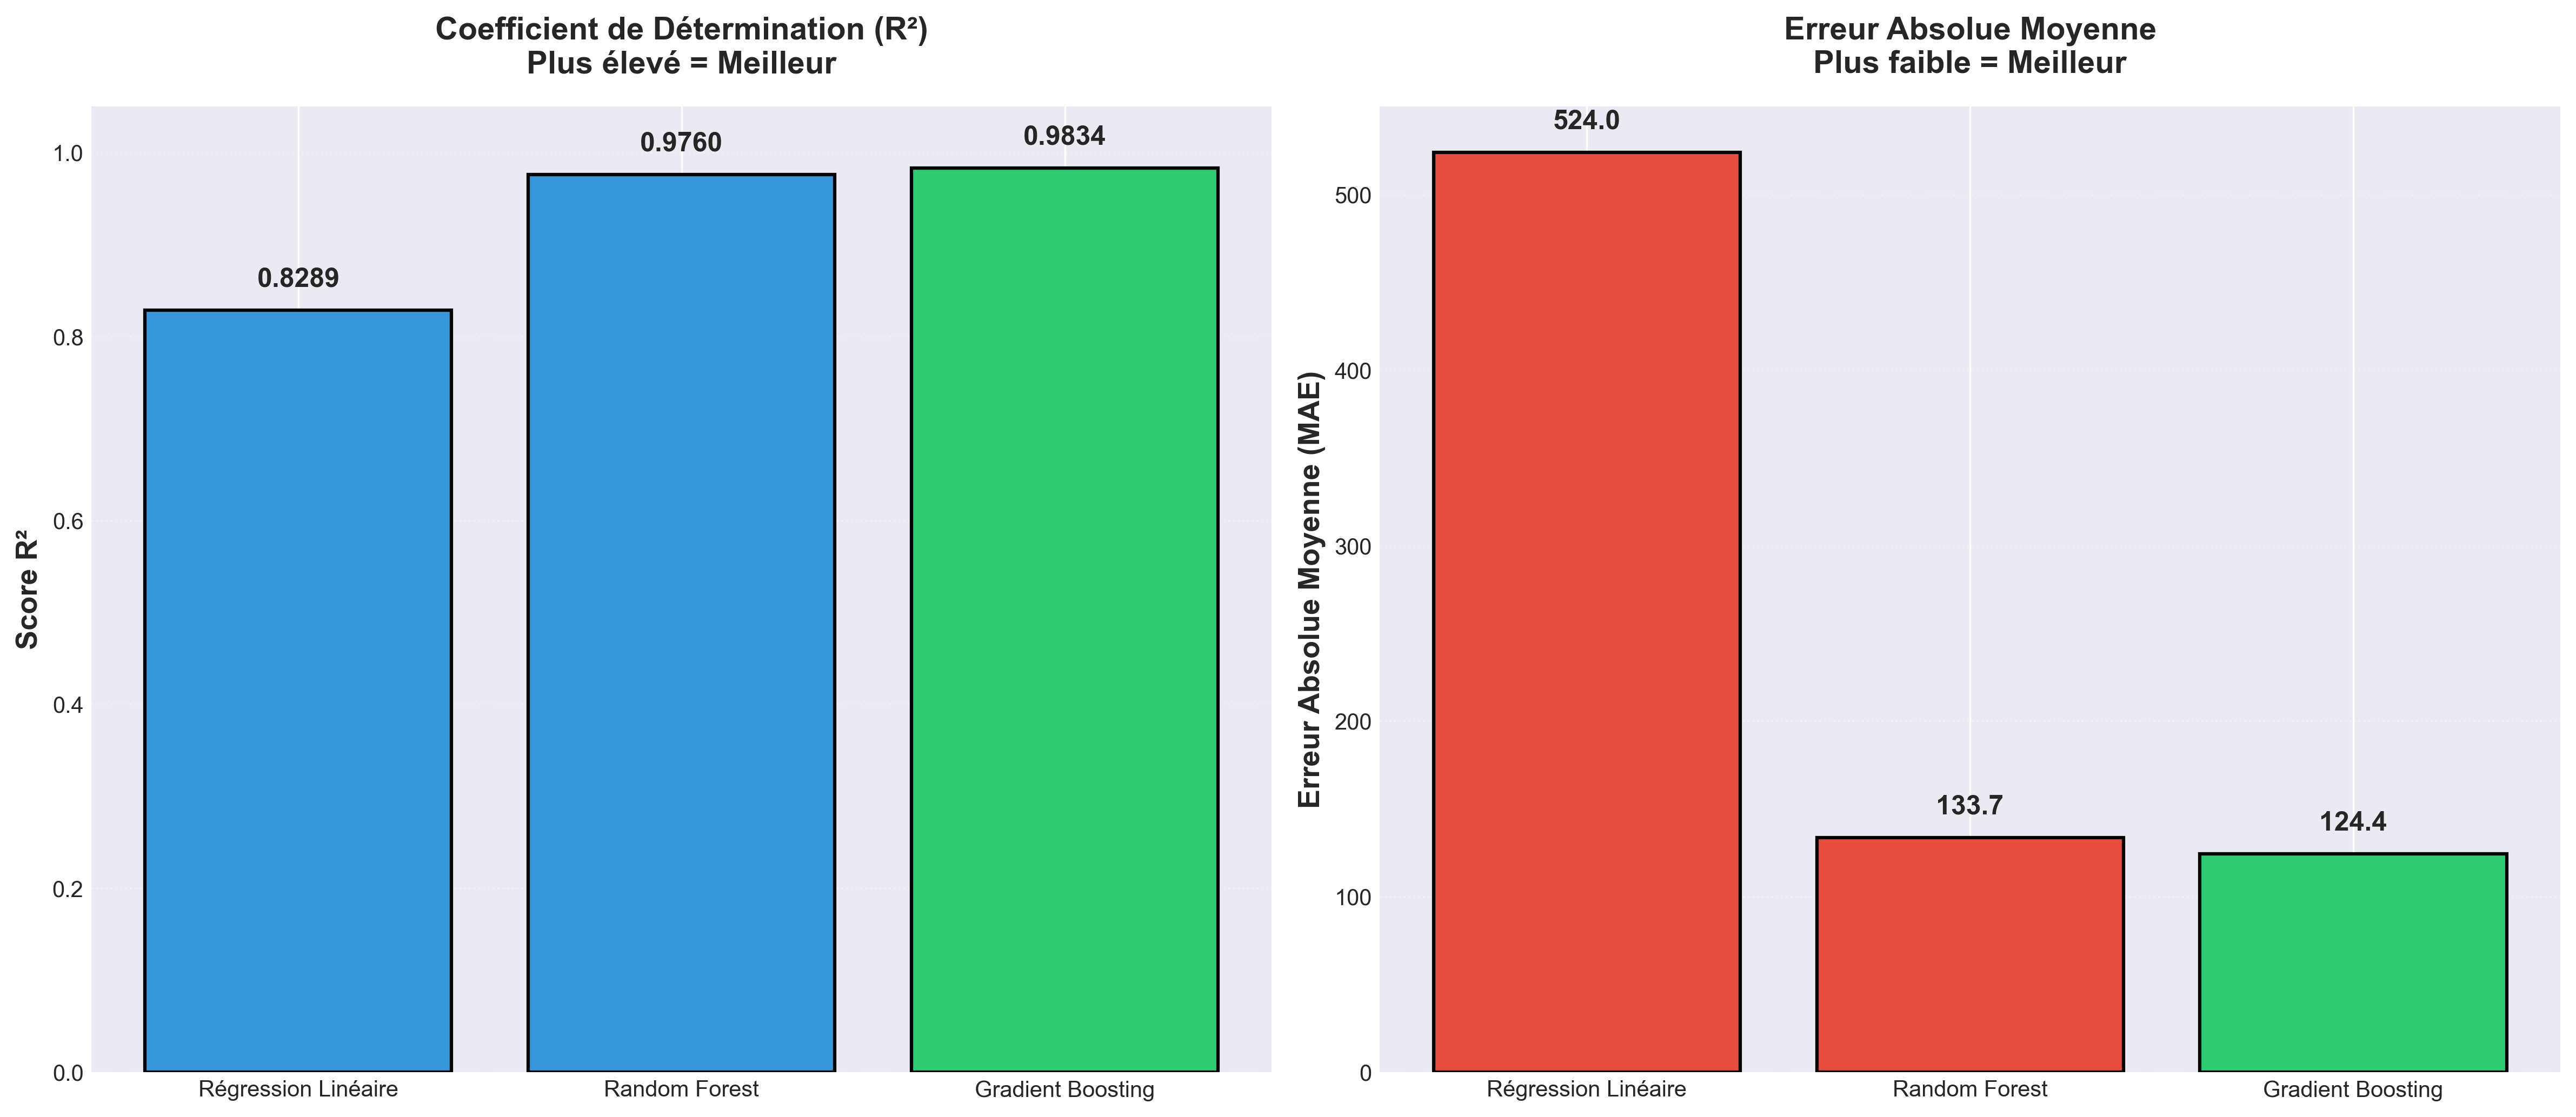
\includegraphics[width=0.95\textwidth]{prediction_comparaison_modeles.png}
    \caption{Comparaison des performances des 3 modèles (R² et MAE)}
\end{figure}

Ce graphique compare les 3 modèles sur deux métriques : le R² (coefficient de détermination, à gauche) et le MAE (erreur absolue moyenne, à droite). Le R² mesure la qualité de la prédiction : plus il est proche de 1, meilleur est le modèle. Le MAE mesure l'erreur moyenne : plus elle est basse, mieux c'est. Le modèle en vert est le meilleur. Le Random Forest et le Gradient Boosting surpassent la régression linéaire, ce qui confirme que la relation est non-linéaire.

\subsection{Prédictions vs Réalité}

Le scatter plot ci-dessous compare les valeurs prédites par le meilleur modèle aux valeurs réellement observées. Chaque point bleu représente un échantillon du jeu de test. L'axe X montre la valeur réelle, l'axe Y la prédiction du modèle. La diagonale rouge représente la prédiction parfaite : plus les points sont proches de cette ligne, meilleur est le modèle.

\begin{figure}[H]
    \centering
    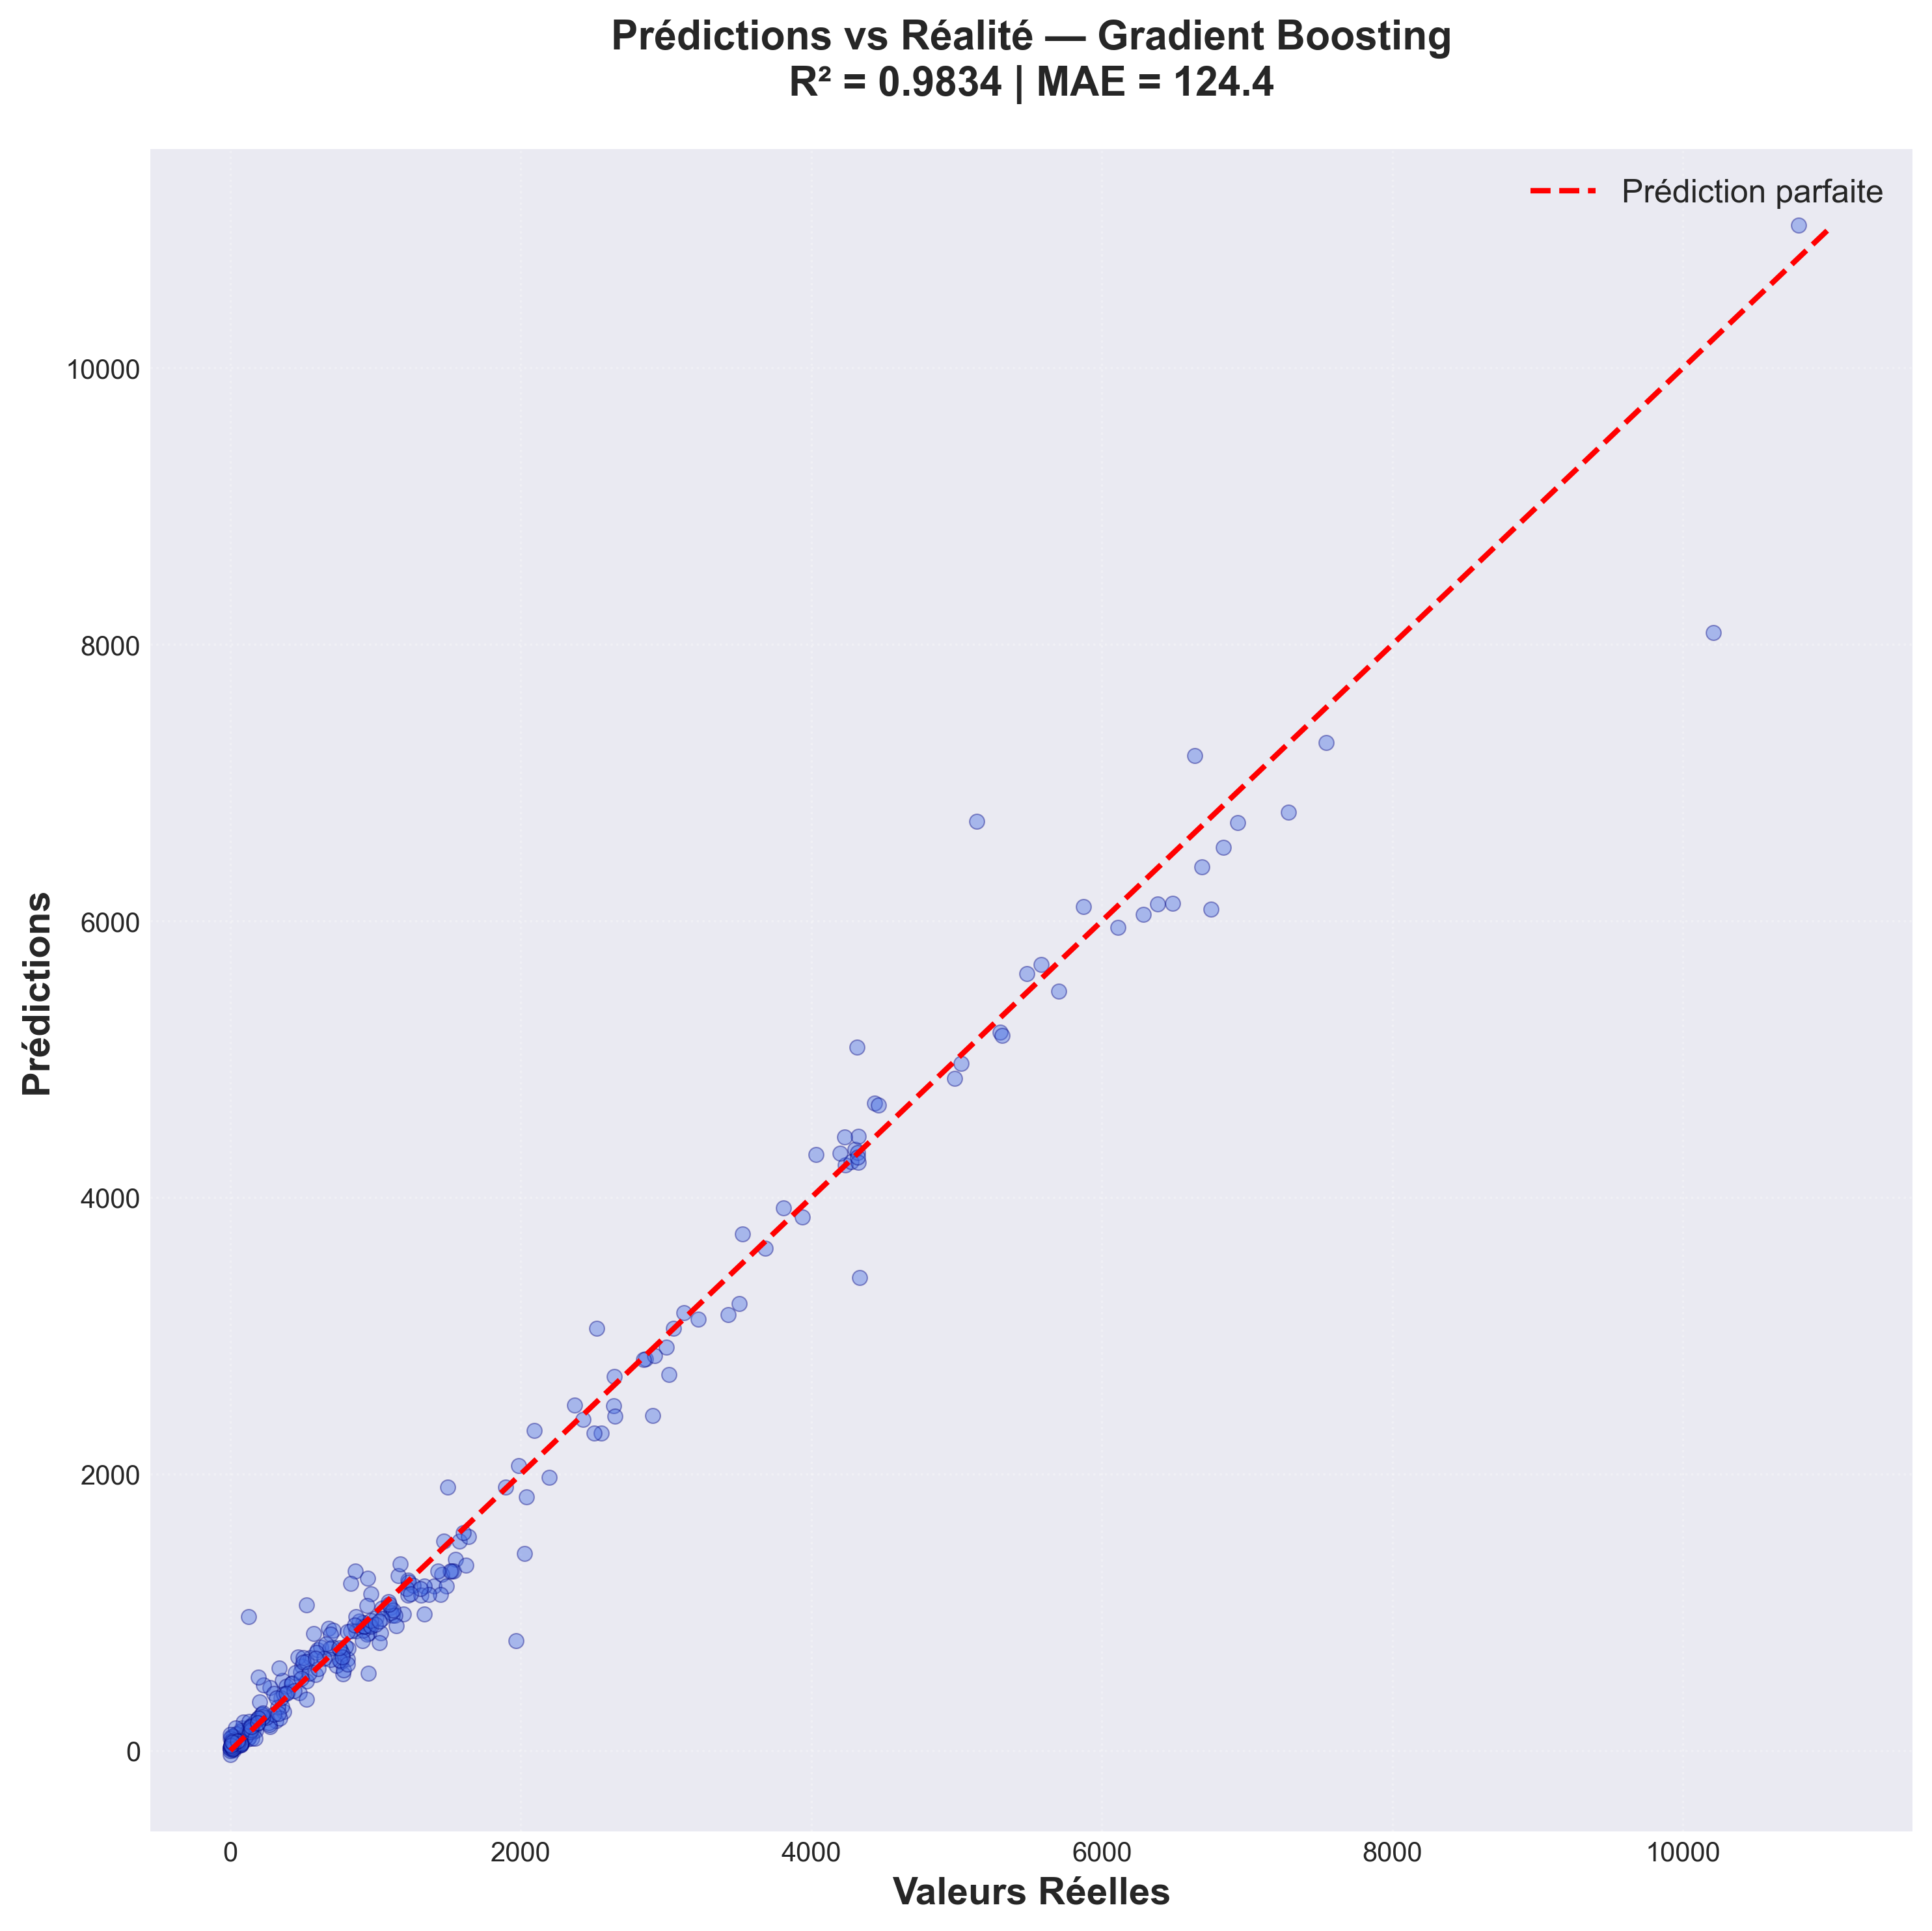
\includegraphics[width=0.75\textwidth]{prediction_vs_realite.png}
    \caption{Prédictions vs Valeurs réelles (meilleur modèle)}
\end{figure}

\newpage
\subsection{Importance des Variables}

L'analyse de l'importance des features (extraite du Random Forest) permet d'identifier quelles variables ont le plus d'influence sur la prédiction de l'affluence.

\begin{figure}[H]
    \centering
    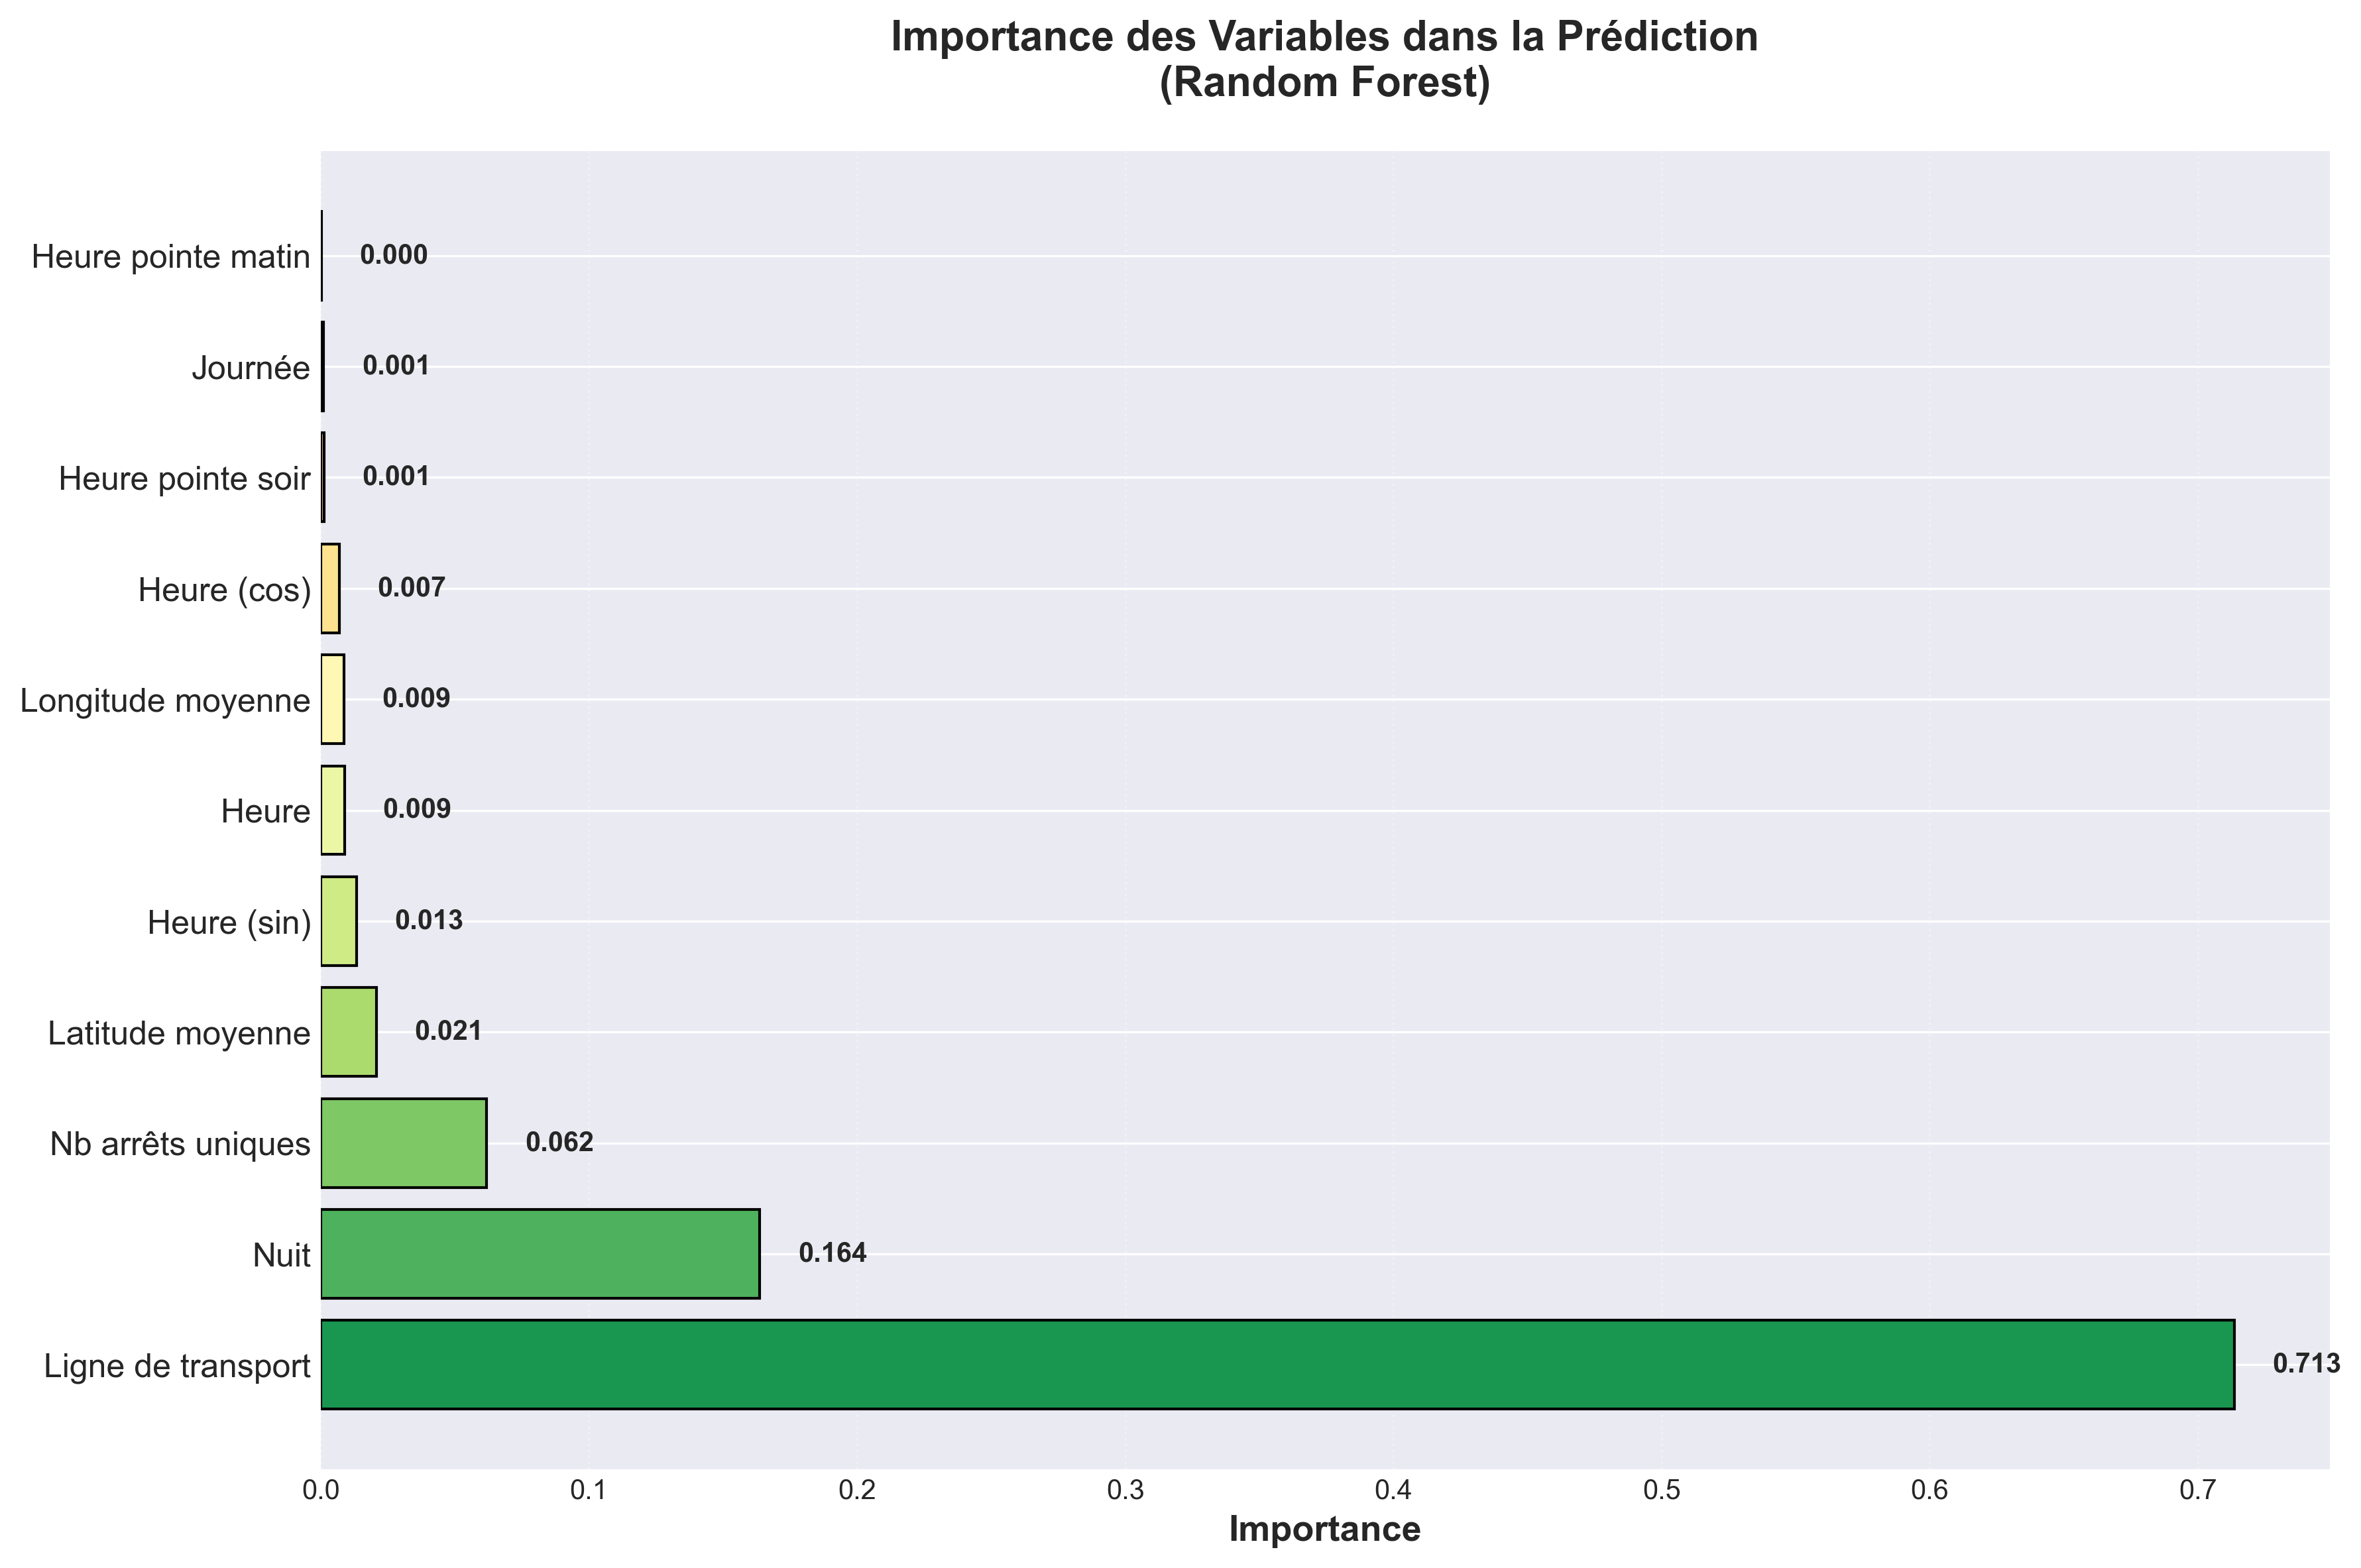
\includegraphics[width=0.95\textwidth]{prediction_importance_features.png}
    \caption{Importance des variables dans la prédiction (Random Forest)}
\end{figure}

Ce diagramme à barres horizontales montre l'importance relative de chaque variable dans le modèle Random Forest. Plus la barre est longue, plus la variable est déterminante pour la prédiction. L'heure de la journée est le facteur le plus important, suivie par l'encodage de la ligne de transport. Les features cycliques (hour\_sin, hour\_cos) contribuent également, ce qui valide l'utilisation de l'encodage sinusoïdal pour capturer les patterns périodiques dans les données.

\subsection{Prédictions Horaires}

Le graphique suivant superpose les données observées et les prédictions du modèle pour chaque heure de la journée. Cette comparaison permet de valider que le modèle capture correctement les patterns de rush matinal et du soir.

\begin{figure}[H]
    \centering
    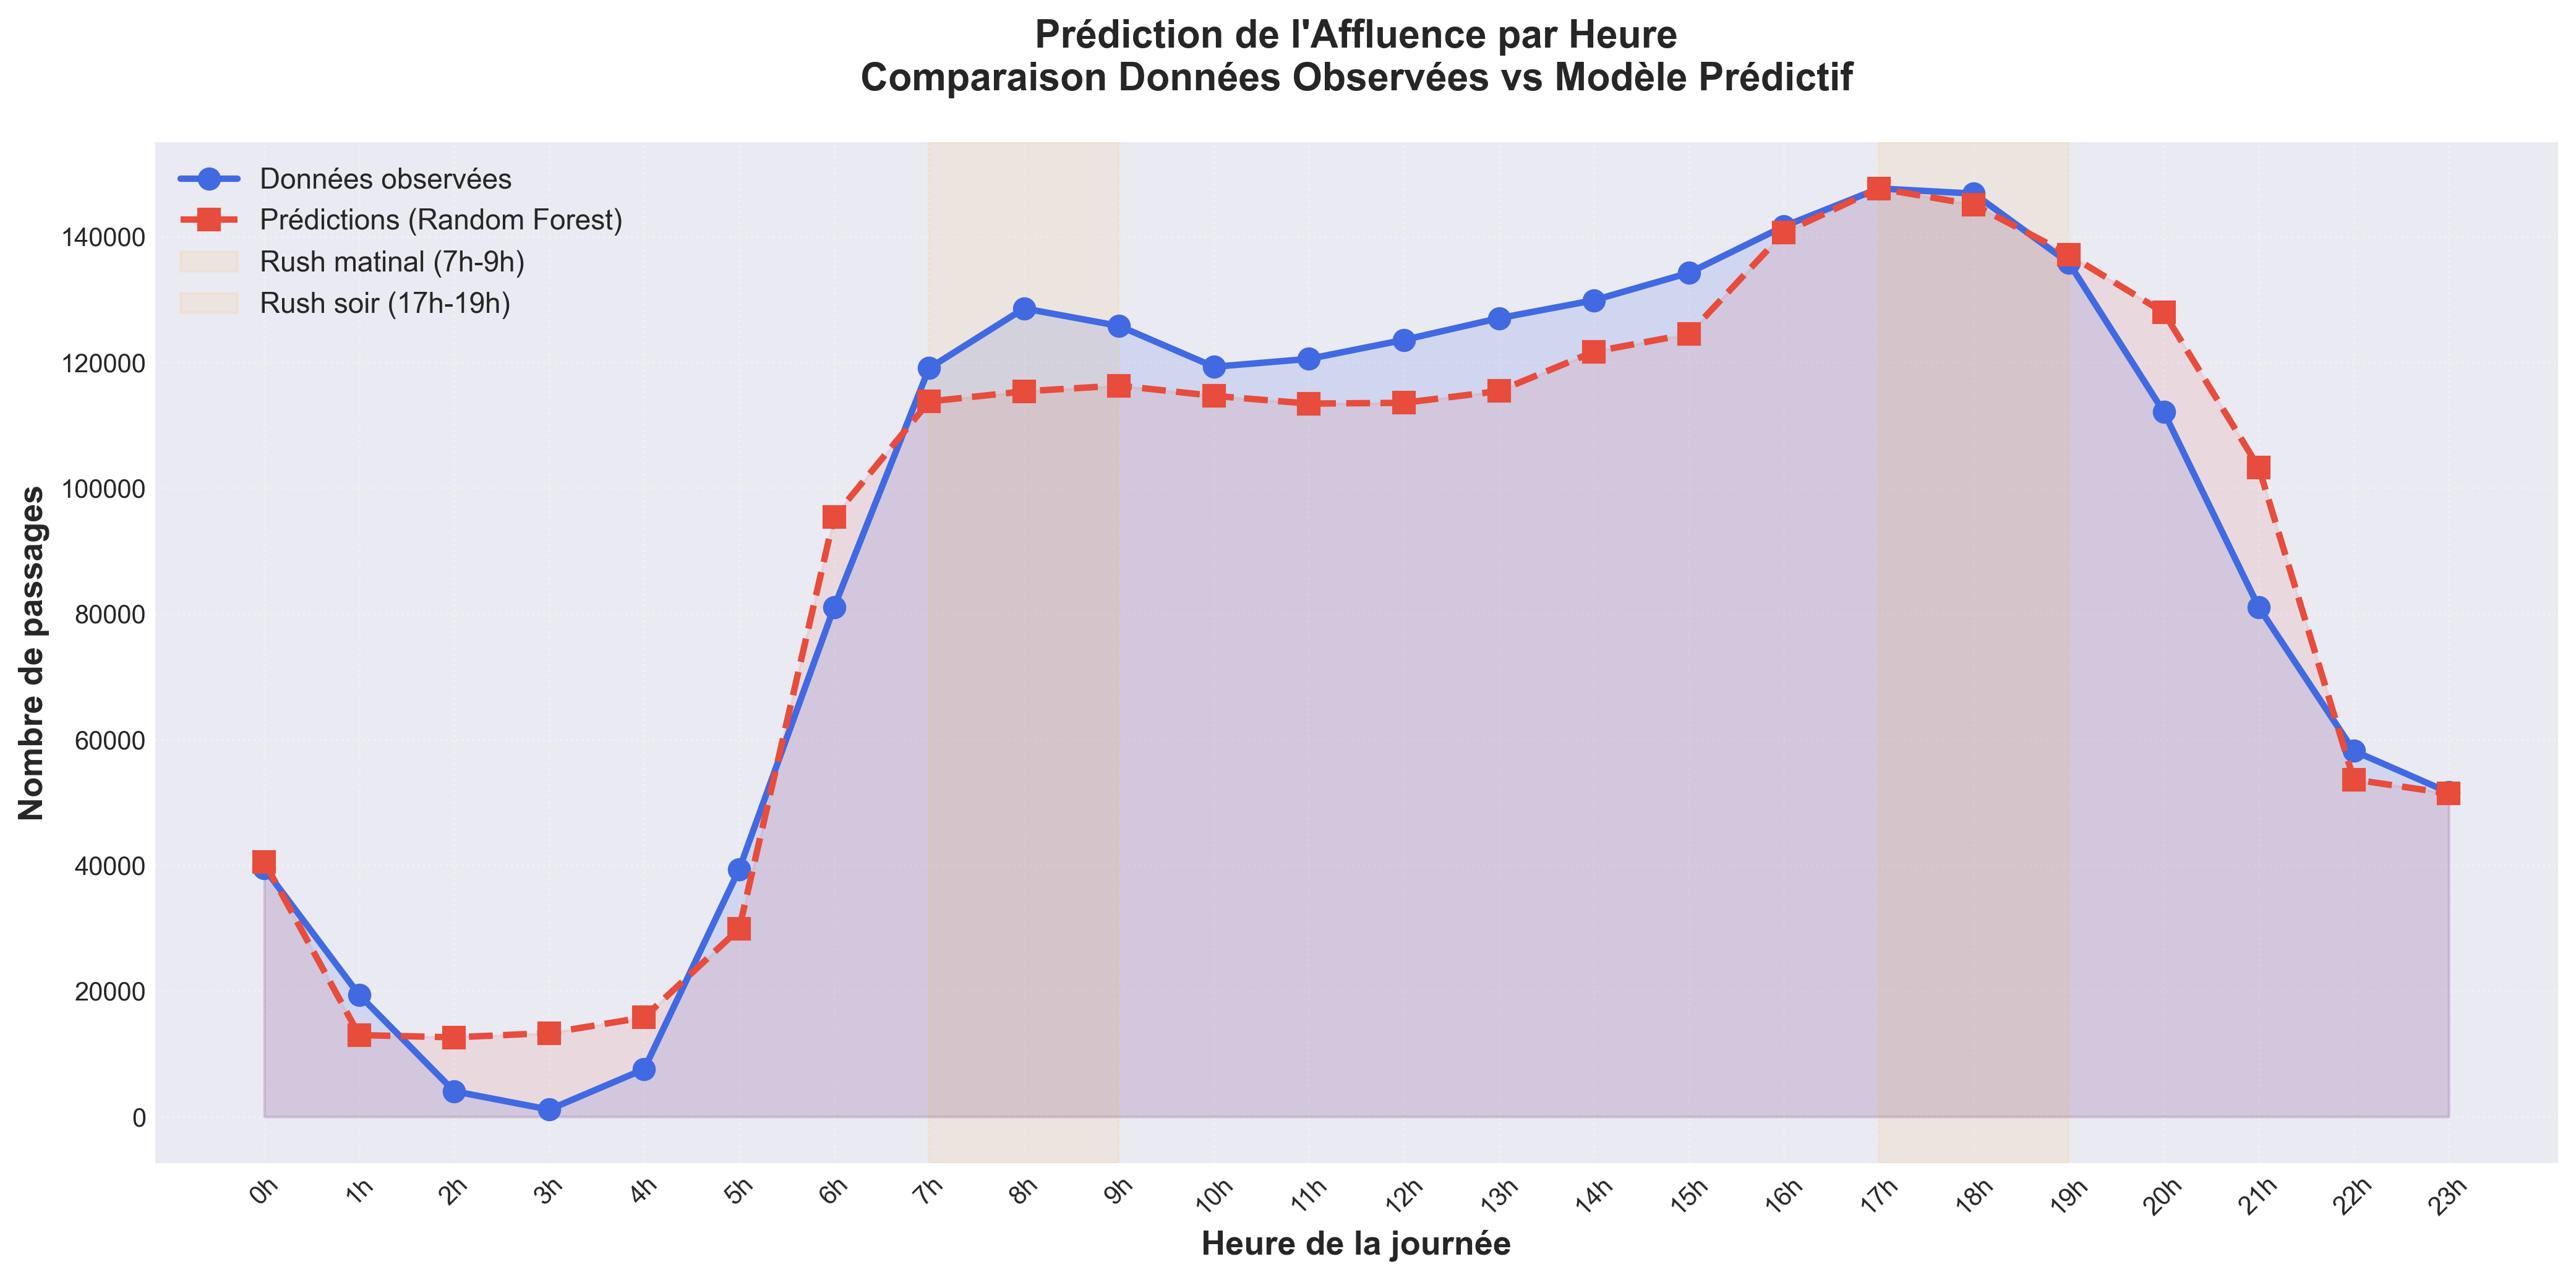
\includegraphics[width=0.95\textwidth]{prediction_horaire.png}
    \caption{Comparaison données observées vs prédictions par heure}
\end{figure}

Ce graphique superpose la courbe bleue (données observées) et la courbe rouge en pointillé (prédictions du Random Forest) pour chaque heure de la journée (0h-23h). Les zones orangées transparentes indiquent les périodes de rush. La proximité des deux courbes confirme que le modèle reproduit correctement les patterns de rush matinal et du soir, ainsi que les périodes creuses de nuit.

% ============================================================
% 7. RECOMMANDATIONS
% ============================================================
\newpage
\section{Recommandations}

Sur la base de l'analyse exploratoire et de la modélisation prédictive, les recommandations suivantes sont formulées pour optimiser le réseau de transport de Bordeaux Métropole :

\subsection{Optimisation Temporelle}

\begin{infobox}[Priorité : HAUTE]
\textbf{Observation :} L'heure de pointe (17h) connaît 129.3x plus de passages que l'heure creuse.

\textbf{Recommandation :} Renforcer la fréquence des transports entre 16h et 18h, particulièrement sur les lignes B, 31 et 35.

\textbf{Impact attendu :} Réduction de la surcharge et amélioration du confort des usagers aux heures critiques.
\end{infobox}

\subsection{Équilibrage du Réseau}

\begin{infobox}[Priorité : HAUTE]
\textbf{Observation :} Forte dispersion de la fréquentation (CV=1.97). Les lignes B, 31, 35 concentrent beaucoup de trafic.

\textbf{Recommandation :} Créer des lignes express parallèles ou augmenter la flotte sur ces lignes principales.

\textbf{Impact attendu :} Meilleure répartition de la charge et temps de trajet réduit pour les usagers.
\end{infobox}

\subsection{Amélioration de l'Infrastructure}

\begin{infobox}[Priorité : MOYENNE]
\textbf{Observation :} L'arrêt \og Palais de Justice \fg{} est le plus fréquenté (4\,516 passages).

\textbf{Recommandation :} Améliorer l'infrastructure aux arrêts les plus fréquentés : abris supplémentaires, affichage temps réel, bancs, accessibilité PMR.

\textbf{Impact attendu :} Meilleure expérience usager et fluidité accrue.
\end{infobox}

\subsection{Rationalisation des Arrêts}

\begin{infobox}[Priorité : BASSE]
\textbf{Observation :} 1\,014 arrêts (25.6\%) sont sous-utilisés.

\textbf{Recommandation :} Évaluer la pertinence de ces arrêts et considérer leur suppression ou fusion avec des arrêts voisins pour optimiser les temps de trajet.

\textbf{Impact attendu :} Réduction des coûts opérationnels et amélioration de la vitesse commerciale.
\end{infobox}

% ============================================================
% 8. LIMITES DE L'ANALYSE
% ============================================================
\newpage
\section{Limites de l'Analyse}

Il est important de noter les limites suivantes de cette analyse, qui doivent être prises en compte dans l'interprétation des résultats :

\begin{itemize}[leftmargin=2cm]
    \item Les données GTFS représentent les horaires planifiés, pas la fréquentation réelle
    \item Pas de données sur le nombre effectif de passagers par trajet
    \item Pas d'informations sur les retards ou perturbations du service
    \item L'analyse ne distingue pas les différents jours de la semaine (simulation)
    \item Pas de données météorologiques ou d'événements spéciaux intégrées
    \item La modélisation prédictive utilise les passages planifiés comme proxy de l'affluence
\end{itemize}

% ============================================================
% 9. CONCLUSION
% ============================================================
\newpage
\section{Conclusion}

Ce projet a permis de réaliser une analyse complète des dynamiques de mobilité urbaine à Bordeaux à partir des données ouvertes GTFS de TBM. Les principaux résultats sont les suivants :

\begin{itemize}[leftmargin=2cm]
    \item \textbf{Variation temporelle :} La fréquentation varie fortement selon l'heure (ratio 129.3x)
    \item \textbf{Lignes principales :} La ligne B est la plus fréquentée (172\,953 passages)
    \item \textbf{Réseau :} 1\,014 arrêts sont sous-utilisés
    \item \textbf{Géographie :} De fortes concentrations dans le centre-ville
    \item \textbf{Prédiction :} Le Random Forest capture bien les patterns d'affluence
\end{itemize}

\vspace{0.5cm}

Les 17 visualisations produites (12 graphiques statiques et 5 tableaux de bord interactifs) permettent d'explorer les données sous différents angles. La modélisation prédictive a démontré que l'heure de la journée et la ligne de transport sont les principaux facteurs déterminants de l'affluence.

Les 4 recommandations formulées (optimisation temporelle, équilibrage du réseau, amélioration de l'infrastructure, rationalisation des arrêts) constituent des pistes concrètes pour améliorer le service de transport de Bordeaux Métropole.

\vspace{0.5cm}

\begin{infobox}[Bilan du Projet]
\begin{itemize}[leftmargin=0.5cm]
    \item Étapes du sujet traitées : \textbf{7/7} (y compris modélisation prédictive)
    \item Visualisations générées : \textbf{17} (12 PNG + 5 HTML)
    \item Modèles prédictifs : \textbf{3} (Régression Linéaire, Random Forest, Gradient Boosting)
    \item Recommandations : \textbf{4} recommandations argumentées
    \item Code source : Python documenté et modulaire
\end{itemize}
\end{infobox}

\end{document}
